%
% Adaptive Blind System Identification and Equalization Toolbox for MATLAB
%
% Copyright (C) Imperial College London 2009
%
% Version: $Id: BSIE_Toolbox.tex 425 2011-08-12 09:15:01Z mrt102 $
%
\documentclass[9pt,a4paper,titlepage]{article}
\usepackage{graphicx, amsfonts}
\usepackage{amsmath}
\usepackage{amssymb}
\usepackage{color}
\usepackage{textcomp}
\usepackage{graphicx}
\usepackage{enumitem}
\usepackage{subfigure}
\usepackage{cite}

\usepackage{hyperref}
\hypersetup{
    a4paper,
    bookmarksopen=false,
    bookmarksnumbered=true,
    colorlinks=true,
    citecolor=blue,
    linkcolor=red,
    linktocpage=true,
    linkbordercolor={1 1 1},
    hypertexnames=false,
    plainpages=true,
    pdftitle={Adaptive Blind System Identification and Equalization Toolbox for MATLAB},
    pdfauthor={E.A.P. Habets}
}

\usepackage{listings}
\lstset{
    tabsize=4,
	rulecolor=,
	language=matlab,
    basicstyle=\small \ttfamily,
    upquote=true,
    aboveskip={1.5\baselineskip},
    belowskip={1.5\baselineskip},
    columns=fixed,
    showstringspaces=false,
    extendedchars=true,
    breaklines=true,
    prebreak = \raisebox{0ex}[0ex][0ex]{\ensuremath{\hookleftarrow}},
    frame=none,
    showtabs=false,
    showspaces=false,
    showstringspaces=false,
    identifierstyle= \ttfamily,
    keywordstyle= \color[rgb]{0,0,1},
    commentstyle= \color[rgb]{0.133,0.545,0.133},
    stringstyle= \color[rgb]{0.627,0.126,0.941},
}

%\newcommand{\dfrac}[2]{\frac{\displaystyle #1}{\displaystyle #2}}
%\newcommand{\eqnspc}{\vspace{-5pt}}
\addtolength{\hoffset}{-1cm} \addtolength{\textwidth}{2cm}
\addtolength{\voffset}{-1cm}\addtolength{\textheight}{2cm}

\begin{document}\sloppy

\def\d{{\mathbf d}}
\def\D{{\mathbf D}}
\def\e{{\mathbf e}}
\def\F{{\mathbf F}}
\def\g{{\mathbf g}}
\def\G{{\mathbf G}}
\def\h{{\mathbf h}}
\def\hh{{\widehat{\mathbf h}}}
\def\w{{\mathbf w}}
\def\A{{\mathbf A}}
\def\B{{\mathbf B}}
\def\H{{\mathbf H}}
\def\I{{\mathbf I}}
\def\W{{\mathbf W}}
\def\x{{\mathbf x}}
\def\X{{\mathbf X}}
\def\N{{\mathbf N}}
\def\S{{\mathbf S}}

\title{Adaptive Blind System Identification and Equalization Toolbox for MATLAB\\\vspace{1cm}Version 1.2}

\author{Emanu\"{e}l A.P. Habets, Xiang (Shawn) Lin, Wancheng Zhang,\\Andy Khong, Nikolay D. Gaubitch, Patrick A. Naylor}

\maketitle

\tableofcontents

\newpage
\section*{Abstract}
%Recently, the use of adaptive algorithms for blind system identi�cation in speech dereverberation has been proposed. 
This report provides an introduction to blind system identification and system equalization, and describes  a MATLAB toolbox that contains state-of-the-art blind system identification and system equalization algorithms, performance evaluation methods and analyses tools. In this report, we focus on single-input multiple-output (SIMO) acoustic systems. 

In the first part of this report, background information on blind system identification and system equalization is provided. Here we focus on blind system identification methods that jointly minimize the cross-relation error between different pairs of sensor signals.  In addition, it is shown that an estimate of the (unknown) source signal can be obtained by equalizing the acoustic system. In the second part of this report, a variety of adaptive blind system identification algorithms are described that minimize the total cross-relation error, either in the time or frequency domain. In the third part of this report, varies algorithms are described that can be used to compute the equalization system given the estimated impulse responses of the acoustic system. Finally, we describe performance evaluation methods and analysis tools that are commonly used in this context.

\newpage
\section{Introduction}
\label{chap:literature_review}

\subsection{Literature Overview}
The idea of blind system identification (BSI) was first introduced to the communications community by Sato with the intention of designing efficient communication systems that did not require a training phase \cite{Sato1975}. From that point on, BSI has become an extremely active topic of research, and has been widely applied to various areas such as communications \cite{Giannakis2000}, geophysics, underwater communications \cite{Lee2002}, and multimedia signal processing \cite{Abed-Meraim1997b, Luo1998}. In contrast to non-blind system identification where a known signal is used to facilitate the identification of the acoustic channel, BSI algorithms only utilize signals received from the output of an unknown system for channel estimation. For the case of speech dereverberation, acoustic channels are first identified blindly using received signals from the microphones. These estimated channels are then used to design equalization filters in order to remove reverberation induced by the acoustic channels. 

BSI methods can generally be classified into two main categories: second order statistical (SOS) and higher order statistical (HOS) methods. Comparisons between SOS and HOS methods have been presented in \cite{Tong1998}. The HOS information of a stochastic process can be described by its $k\mathrm{th}$-order cumulant or its Fourier transform; for $k>2$ is also known as a polyspectrum \cite{Haykin1994, Tugnait2000a}. The HOS information of the system output signals contains the phase information of a non-Gaussian process and can be exploited by the HOS-based algorithms either directly, using the polyspectra method \cite{Pan1988}, or indirectly, using the Bussgang algorithm proposed in \cite{Godfrey1981, Bellini1994}. Because HOS information cannot be accurately computed from a small number of observations, slow convergence is the critical drawback of all existing HOS methods \cite{Huang2006}. In addition, a cost function based on HOS information is, in general, not convex. As a consequence an HOS-based algorithm can converge to a local minimum. In addition, their overall performance is degraded by corrupting noise in the observations. 

Fortunately, these problems can be overcome in multichannel systems such as single-input multiple-output~(SIMO) and multiple-input multiple-output~(MIMO) systems where multiple sensors are employed \cite{Tong1998}. Specifically, SOS information of the system outputs in the form of \textit{cyclostationarity} can be exploited for blind identification, where cyclostationarity indicates the periodicity of the mean and autocorrelation function of a stochastic process \cite{Haykin2002}. By exploiting such periodicity, the preservation of phase information is now possible for processes that are wide-sense cyclostrationary. The use of cyclostationarity for recovering the amplitude and phase of the channel response was first recognized in \cite{Gardner1991}, and was formally developed in the context of BSI  in \cite{Tong1991} based on the spatial diversity obtained from multiple channels. Since then, a large number of SOS-based multichannel BSI algorithms have been developed \cite{Tong1998, Loubaton2000}, among which celebrated work includes the cross-relation~(CR) method \cite{Liu1993, Tong1994, Tong1995, Gurelli1995, Xu1995}, the subspace method \cite{Moulines1995}, the LP-based subspace algorithm \cite{Slock1994}, and the two-step maximum likelihood algorithm \cite{Hua1996}. These methods utilize either the cyclostationarity of the received signals or spatio-temporal diversity of the multichannel systems to achieve successful BSI up to a non-zero arbitrary scale factor using only the SOS of the multiple outputs \cite{Abed-Meraim1997b, Giannakis2000}. In this report, only SOS-based BSI algorithms are considered.

Recent advances and innovations in speech communications have led to increased interest in acoustic signal processing aiming at extracting and interpreting information from acoustic signals in, for example, the cocktail party situation \cite{Huang2005a, Huang2006}. As a result, accurately identifying acoustic systems has become the main issue in the literature for the study of how acoustic signals are transmitted and distorted. This has motivated the adoption of BSI techniques into the acoustic signal processing community, where speech source separation and speech dereverberation are two important research topics. However, such adoption is not straightforward due to the substantial differences between communication systems and acoustic systems \cite{Benesty2008}. Traditionally, antenna arrays for wireless communications work in a fairly open space. Typical channel impulse responses are much shorter than acoustic impulse responses. For example, a typical office or living room exhibits reverberation time $T_{60}$ in the order of 50 to 600~ms. At a sample frequency of 8~kHz, the acoustic impulse responses are around 400 to 4800 coefficients long.  In addition, human hearing has an extremely wide dynamic range and is very sensitive to the audible effect caused by the tail of the acoustic impulse response.  Undoubtedly, these facts have created great challenges for well-established classic BSI algorithms in terms of computational complexity and identification accuracy \cite{Benesty2001, Huang2006, Huang2006a}.

Nevertheless, promising progress has been made in the acoustic signal processing community as several batch and adaptive algorithms have been developed for blind identification of SIMO acoustic systems \cite{Huang2002, Huang2003, Gannot2003, Benesty2004a, Huang2005}. These algorithms can accurately determine the impulse responses of an identifiable multichannel system using a finite number of samples when additive noise in the system outputs is weak. Among these algorithms, batch algorithms are difficult to implement in an adaptive mode and are computationally expensive given the high order nature of acoustic impulse responses \cite{Huang2006a}. In addition, their performance relies on the existence of 
numerically well-defined dimensions of the signal or noise subspace. Adaptive algorithms, in contrast, are easier to implement and are suitable for real-time applications. They are also capable of tracking the dynamic nature of acoustic impulse responses. However, the overall performance for these algorithms is still unsatisfactory due to various issues, which can be summarized  as follows:
\begin{itemize}
  \item The order of the unknown system is often erroneously assumed to be 
      available \cite{Gannot2003}.
  \item Even with a small amount of noise, most algorithms cannot operate successfully.
  \item The computational burden due to long acoustic impulse responses is still 
      significant even for adaptive algorithms.
  \item The presence of common zeros limits the accuracy and convergence speed of blind 
      identification.
\end{itemize}
These issues have become the subjects of current research in the community \cite{Xu1995, Liu1996, Hua1996, Abed-Meraim1997b, Tong1998, Huang2006, Gaubitch2006c}, and significant contributions have been made to overcome some of them. For example, algorithms have been developed in \cite{Hasan2005, Hasan2006, Ahmad2006, Gaubitch2006b, Ahmad2007} to improve the noise robustness of multichannel least mean squares (MCLMS) and normalized multichannel frequency domain least mean squares (NMCFLMS) algorithms \cite{Huang2002, Huang2003}. Additionally, system order estimation was investigated in \cite{Gurelli1995, Liavas1999a}.

System equalization aims to recover the anechoic source signal from the sensor signals by equalizing the acoustic system. Since a single acoustic channel is generally considered as a nonminimum phase system \cite{Neely1979}, the infinite impulse response (IIR) causal inverse is unstable, which is not applicable in practice. To equalize a single acoustic channel, a finite impulse response (FIR) least squares (LS) inverse filter can be used \cite{Mourjopoulos1982}. When multiple channels are employed, it is revealed by the multiple-input/output inverse theorem (MINT) that the multichannel acoustic system can be exactly inverted by a set of FIR filters subject to some conditions \cite{Miyoshi1988}. Later, weighted LS inverse systems were used for room acoustics equalization \cite{Hofbauer2005}. More recently, channel shortening (CS) techniques \cite{Melsa1996,Martin2005}, which were firstly exploited in digital communications to mitigate inter-symbol and inter-carrier interferences, were also used for the equalization of acoustic systems \cite{Kallinger2006}.

\subsection{Problem Formulation}
The aim of BSI is to identify unknown system impulse responses excited by unknown source signals. As shown in Fig.~\ref{fig:bsi_diag}, an acoustic environment containing one source and $M$ sensors can be modelled as a linear SIMO system. Each sensor signal results from a source signals which is passed though an acoustic channel. In this report we focus on SIMO systems that can be extended to multi-input multi-output systems as shown in \cite{Huang2006, Huang2006a}. It should also be noted that although acoustic channels are inherently time-varying due to, for example, changes of source-sensor-configurations, we can use FIR filters to model acoustic channels since acoustic systems generally change slowly compared to the length of their channel impulse responses \cite{Huang2006a}. The order of the unknown system is also assumed to be known. Although algorithms such as minimum description length~(MDL) \cite{Rissanen1978} or information theoretic criteria~(AIC) \cite{Akaike1974} can in principle be employed for channel order estimation, they are sensitive to variations in SNR and data sample size \cite{Liavas1999a}. 
\begin{figure}[htbp]
  \begin{center}
    \mbox{
      \subfigure[]{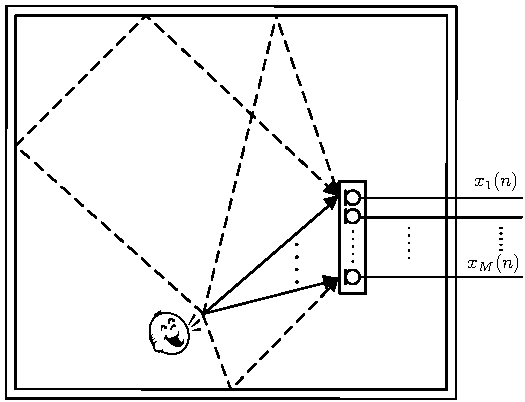
\includegraphics[width=0.475\linewidth]{figs/pdf/room.pdf}\label{fig:room}} \quad
      \subfigure[]{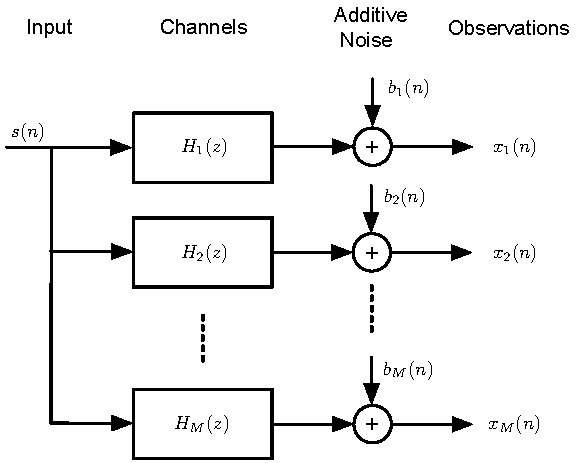
\includegraphics[width=0.475\linewidth]{figs/pdf/system.pdf} \label{fig:system}}
      }
    \caption{Diagram of (a) an $M$-channel SIMO acoustic system, and (b) BSI problem formulation.}
    \label{fig:bsi_diag}
  \end{center}
\end{figure}

For an $M$-channel SIMO system as shown in Fig.~\ref{fig:bsi_diag}, the $m\mathrm{th}$ impulse response with $L$ coefficients can be denoted as
\begin{equation}\label{eqn:bsi_m_impulse_ch_LitRev}
    \mathbf{h}_m \, = \, [h_{m,0}~h_{m,1}~\ldots~h_{m,L-1}]^T,
\end{equation}
for $m=1,2,\ldots,M$, and the $m\mathrm{th}$ microphone signal can be expressed as
\begin{equation} \label{eqn:scalor_in_out_ch_LitRev}
x_m(n) \, = \, \sum_{j=0}^{L-1} h_{m,j} \, s(n-j)+b_m(n),
\end{equation}
where $s(n)$ is the source signal and $b_m(n)$ is the additive noise. The additive noise is assumed to be zero-mean and uncorrelated with the source signal. In vector form,~(\ref{eqn:scalor_in_out_ch_LitRev}) can be
written\footnote{Note that the elements of the signal vectors $\mathbf{x}_m(n)$, $\mathbf{s}(n)$, and $\mathbf{b}_m(n)$ are in time reversed order.}
\begin{equation} \label{eqn:vector_in_out_ch_LitRev}
  \mathbf{x}_m(n) \, = \, \mathbf{H}_m \, \mathbf{s}(n)+\mathbf{b}_m(n),
\end{equation}
where $\mathbf{s}(n)=[s(n)~s(n-1)~\ldots~s(n-2L+2)]^T$, $\mathbf{x}_m(n)=[x_m(n)~x_m(n-1)~\ldots~x_m(n-L+1)]^T$,
$\mathbf{b}_m(n)=[b_m(n)~b_m(n-1)~\ldots~b_m(n-L+1)]^T$, and $\mathbf{H}_m$ is the
$L\times(2L-1)$ convolution matrix for the $m\mathrm{th}$ channel such that
\begin{equation}\label{eqn:ch_LitRev_convolutional_mtx_chm}
  \mathbf{H}_m = \left[%
  \begin{array}{cccccc}
  h_{m,0} & \cdots & h_{m,L-1} & \cdots & \cdots & 0 \\
  0 & h_{m,0} & \cdots & h_{m,L-1} & \cdots & 0 \\
  \vdots & \ddots & \ddots & \ddots & \ddots & \vdots \\
  0 & \cdots & \cdots & h_{m,0} & \cdots & h_{m,L-1} \\
  \end{array}%
  \right].
\end{equation}
Since the impulse responses are assumed to be slowly time-varying, $\mathbf{H}_m$ is independent of $n$. By concatenating all $M$ outputs of~(\ref{eqn:vector_in_out_ch_LitRev}), a system of equations
\begin{equation}\label{eqn:global_in_out_ch_LitRev}
    \mathbf{x}(n) \, = \, \mathbf{H}\mathbf{s}(n)+\mathbf{b}(n)
\end{equation}
can be obtained using the following quantities
\begin{align}
    \mathbf{x}(n)&=[\mathbf{x}_1^T(n)~\mathbf{x}_2^T(n)~\ldots~\mathbf{x}_M^T(n)]^T, \\
    \mathbf{H}&=[\mathbf{H}^T_1~\mathbf{H}^T_2~\ldots~\mathbf{H}^T_M]^T,
    \label{eqn:ch_LitRev_global_channel_mtx}\\
    \mathbf{b}(n)&=[\mathbf{b}_1^T(n)~\mathbf{b}_2^T(n)~\ldots~\mathbf{b}_M^T(n)]^T.
\end{align}
The problem of BSI is to find $\mathbf{h}=[\mathbf{h}_1^T~\mathbf{h}_2^T~\ldots~\mathbf{h}_M^T]^T$ using only $\mathbf{x}(n)$. This means that, with
reference to Fig.~\ref{fig:system}, for a given output $\mathbf{x}(n)$ a
unique solution to $\mathbf{h}$ should be obtained up to a non-zero scale factor across all channels. This scale factor is irrelevant in most of acoustic signal processing applications.

\subsection{Channel Identifiability Conditions}
Channel identifiability is concerned with the existence of a unique solution to the unknown 
system impulse responses with respect to a particular type of system identification 
algorithm \cite{Abed-Meraim1997b}. According to \cite{Xu1995}, two inductive conditions are 
necessary and sufficient for blind identifiability of a SIMO system using BSI algorithms, 
which can be summarized as follows:
\begin{description}
  \item[(C1.1)] \textbf{Channel diversity}: The use of 
      multisensor techniques introduces channel diversity and enables the exploration of 
      SOS of the system outputs for blind identification of SIMO systems \cite{Tong1994, 
      Loubaton2000}. Channel diversity in this context refers to channels being 
      \textit{coprime}, that is, multichannel transfer functions do not share any 
      common zeros. If one or more common zeros exist across all channels then these 
      channels are not coprime. As an extreme example, a SIMO system with $M$ identical 
      channels is of no difference to a single-channel system which exhibits no channel 
      diversity and is thus unidentifiable using BSI algorithms. Most existing 
      methods \cite{Xu1995, Huang2002, Huang2003, Gannot2003} fail to produce a unique 
      solution of channel estimates when common zeros exist since they cannot distinguish 
      the common zeros due to the unknown system from ones due to the source signal.
  \item[(C1.2)] \textbf{Condition for the input signals}: 
      Although BSI algorithms only rely on output signals
  of the system, the characteristics of input signals are not negligible. An
  obvious requirement is that the input data should be non-zero valued. According
  to \cite{Xu1995}, the $L\times L$ Hankel matrix of the source signal given by
  \begin{equation} \label{eqn:hankel_ch_LitRev}
  \mathbf{S}(n) = \left[%
  \begin{array}{cccc}
  s(n) & s(n-1) & \cdots & s(n-L+1)  \\
  s(n-1) & s(n-2) & \cdots & s(n-L)  \\
  \vdots & \vdots & \ddots & \vdots  \\
  s(n-L+1) & s(n-L) & \cdots & s(n-2L+2)  \\
  \end{array}%
  \right]
  \end{equation}
  must be of full-rank. This can be understood by expressing,
  \begin{equation}\label{eqn:hankel_cond_ch_LitRev}
    \mathbf{S}(n)\mathbf{h}_m \, = \, \mathbf{x}_m(n), \qquad m=1,2,\ldots,M
  \end{equation}
  for the noiseless case, from which it can be found that if $\mathbf{S}(n)$ is rank
  deficient,~(\ref{eqn:hankel_cond_ch_LitRev}) will not lead to a unique solution even if
  the source signal $s(n)$ is known since there are insufficient number of linear
  equations to solve all unknown coefficients of $\mathbf{h}_m$. In other words, a
  rank-deficient $\mathbf{S}(n)$ can not fully excite any SIMO system.
\end{description}
The channel identifiability conditions have been studied in \cite{Tugnait1995, Ding1996, Hua1996a, Reddy1997, Serpedin1999} and extended to MIMO case in \cite{Hua2000}. 

\subsection{Cross-Relation Method}
As one of the first proposed SOS-based multichannel BSI algorithms, the CR method \cite{Xu1995} has served as the foundation for many subsequent algorithms.  Using (\ref{eqn:scalor_in_out_ch_LitRev}) and assuming that $b_m(n)=0 \; \forall m$, we can derive the fact that
\begin{equation}\label{eqn:CR_scalor_ch_LitRev}
    x_m(n)* h_l \, = \, s(n)* h_m * h_l \, = \, x_l(n) * h_m, \qquad
    m,l = 1,2,\ldots,M,~m \neq l.
\end{equation}
In vector form,~(\ref{eqn:CR_scalor_ch_LitRev}) can be expressed as
\begin{equation}\label{eqn:CR_ch_LitRev}
    \mathbf{x}_m^T(n)\mathbf{h}_l \, = \, \mathbf{x}_l^T(n)\mathbf{h}_m, \qquad
    m,l = 1,2,\ldots,M,~m \neq l,
\end{equation}
where $h_l$ and $h_m$ denote the $l$th and $m$th acoustic impulse responses, respectively. Multiplying~(\ref{eqn:CR_ch_LitRev}) by $\mathbf{x}_m(n)$ and taking the expectation on both sides leads to
\begin{equation}\label{eqn:CR_crosscorr_ch_LitRev}
    \mathbf{R}_{x_mx_m}\mathbf{h}_l \, = \, \mathbf{R}_{x_mx_l}\mathbf{h}_m, \qquad
    m,l = 1,2,\ldots,M,~m \neq l.
\end{equation}
where $\mathbf{R}_{x_mx_l}$ is the cross-correlation matrix between $\mathbf{x}_m(n)$ and
$\mathbf{x}_l(n)$ given by
\begin{equation}\label{eqn:crosscorr_ch_LitRev}
     \mathbf{R}_{x_mx_l} \, = \, \mathrm{E}\{\mathbf{x}_m(n)\mathbf{x}^T_l(n)\}.
\end{equation}
The relation described by (\ref{eqn:CR_crosscorr_ch_LitRev}) results in $M(M-1)$ distinct equations. Summing~(\ref{eqn:CR_crosscorr_ch_LitRev}) over $M-1$ cross-relations associated with one particular channel $\mathbf{h}_m$ results in
\begin{equation}\label{eqn:CR_overall}
    \sum^{M}_{m = 1,~m \neq l}\mathbf{R}_{x_mx_m}\mathbf{h}_l \, = \,
    \sum^{M}_{m = 1,~m \neq l}\mathbf{R}_{x_mx_l}\mathbf{h}_m, \quad m=1,\ldots,M.
\end{equation}
For $m=1,\ldots,M$ we then have a total of M equations that can be expressed in matrix form as
\begin{equation} \label{eqn:CR_overallM_ch_LitRev}
    \mathbf{R}\mathbf{h} \, = \, \mathbf{0}_{[ML\times 1]}
\end{equation}
with
\begin{equation} \label{eqn:corrmatrix}
  \mathbf{R} = \left[%
  \begin{array}{cccc}
  \displaystyle\sum_{m \neq 1}\mathbf{R}_{x_mx_m} & -\mathbf{R}_{x_2x_1} & \cdots & -\mathbf{R}_{x_Mx_1} \\
  -\mathbf{R}_{x_1x_2} & \displaystyle\sum_{m \neq 2}\mathbf{R}_{x_mx_m} & \cdots & -\mathbf{R}_{x_Mx_2} \\
  \vdots & \vdots & \ddots & \vdots \\
  -\mathbf{R}_{x_1x_M} & -\mathbf{R}_{x_2x_M} & \cdots & \displaystyle\sum_{m \neq M}\mathbf{R}_{x_mx_m} \\
\end{array}%
\right]_{[ML \times ML]}
\end{equation}
\begin{equation}
  \mathbf{h} = [\mathbf{h}_1^T,~\mathbf{h}_2^T,~\ldots,~\mathbf{h}_M^T]^T, \label{eqn:concat_h}
\end{equation}
and $\mathbf{0}_{ML\times 1}$ is a $ML\times 1$ null vector. If the channel identifiability conditions are satisfied, the rank of $\mathbf{R}$ is $ML-1$, and the solution to $\mathbf{h}$ lies within the null space of $\mathbf{R}$ \cite{Xu1995,Avendano1999}.

For the noisy cases, i.e. $b_m(n) \neq 0,~\forall m$,~(\ref{eqn:CR_overallM_ch_LitRev}) must be rewritten \cite{Huang2002}
\begin{equation}\label{eqn:subspace_err_ch_LitRev}
    \mathbf{R}\mathbf{h} \, = \, \mathbf{e}.
\end{equation}
The latter expression can be used to define a cost function
\begin{equation}\label{eqn:costfunc_subspace_ch_LitRev}
   J = \|\mathbf{e}\|^2_2 \, = \, \mathbf{e}^T\mathbf{e}.
\end{equation}
Correspondingly, $\mathbf{\widehat{h}}$ can be obtained by
minimizing~(\ref{eqn:costfunc_subspace_ch_LitRev}) in the LS sense, that is,
\begin{equation}\label{eqn:min_costfunc_subspace_ch_LitRev}
    \mathbf{\widehat{h}} \, = \, \arg\min_{\mathbf{h}}\mathbf{h}^T\mathbf{R}^T\mathbf{R}\mathbf{h},
\end{equation}
where $\mathbf{\widehat{h}}$ can be found from eigenvectors of $\mathbf{R}$ associated with the smallest eigenvalue. It is worthwhile noting that~(\ref{eqn:costfunc_subspace_ch_LitRev}) does not necessarily lead to a noise-robust solution to $\mathbf{h}$ as indicated in \cite{Hasan2006}.

\subsection{Hierarchy of the Toolbox}
As illustrated in Fig.~\ref{fig:structure}, the toolbox functions are divided into four categories:
\begin{enumerate}
\item Blind System Identification
\begin{enumerate}
\item Initialization
\item Algorithms
\end{enumerate}
\item System Equalization
\item Performance Evaluation and Analyses
\item Auxiliary
\end{enumerate}

\begin{figure}[htbp]
  \begin{center}
   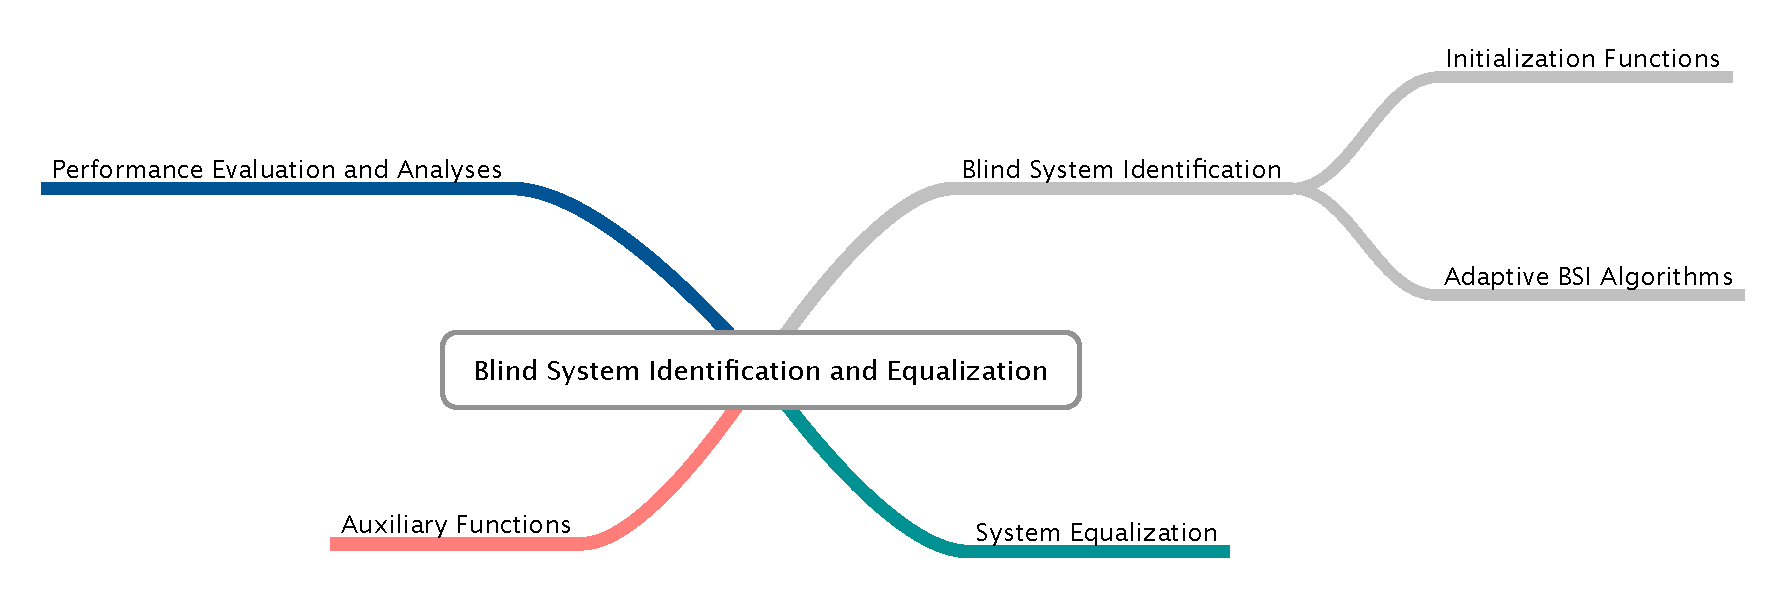
\includegraphics[width=\linewidth]{figs/pdf/structure.pdf}
    \caption{Structure of the BSIE toolbox for MATLAB}
    \label{fig:structure}
  \end{center}
\end{figure}

%
% Blind System Identification
%
\section{Blind System Identification}
% Introduction
In this Section various blind system identification algorithms are described. All algorithms are based on minimizing the so-called cross-relation error \cite{Huang2002}. Both time- and frequency domain algorithms are described including an example script. Currently, only adaptive algorithms are incorporated in the toolbox.

% Multichannel LMS algorithm
\subsection{Multichannel LMS algorithm:~mclms()}

\begin{enumerate}[font=\bf, labelindent=\parindent, widest=123456789012, leftmargin=*, align=left]
\item[Purpose] Time-domain multichannel LMS adaptive filtering algorithm for blind system identification.
	
\item[Syntax] \verb"[h_hat, xin] = init_mclms(L, N, M, h_hat0, xin0)"

The input and output parameters of \verb"init_mclms()" are summarized below.

\vspace{-.5em} \begin{verbatim}
Input Parameters [size]:
       L       : filter length
       M       : number of channels
       xin0    : initial input matrix [L x M]
       h_hat0  : initial filter coef. matrix 
                 (unit-norm constrained) [L x M]

Output parameters [size]:
       xin     : initialized signal matrix [L x M]
       h_hat   : initialized filter coef. matrix [L x M]
\end{verbatim}

\verb"[h_hat, J] = mclms(xin, h_hat, mu, ss_cntr)" 
	
The input and output parameters of \verb"mclms()" for an FIR adaptive filter of $L$ coefficients are summarized below.

\vspace{-.5em} \begin{verbatim}
Input Parameters [size]:
       xin     : input vector [N x M]
       h_hat   : current filter coef. matrix [L x M]
       mu      : step-size
       ss_cntr : type of step-size control 
                 (optional: default `normalized'):
                 `fixed' - fixed with unit-norm-constrained;
                 `vss' - variable step-size

Output parameters [size]:
       h_hat   : updated filter coef. matrix [L x M]
       J       : value of cost function
\end{verbatim}

\item[Description] \verb"mclms()" is a classic time-domain multichannel adaptive algorithm (with unit-norm constraint)  for blind system identification based on the cross-relation~(CR) \cite{Huang2002}. \verb"mclms()" takes the observed microphone signals $\mathbf{x}(n)$, the length of the room impulse responses $L$, the step size $\mu$, the true room impulse responses $\mathbf{h}$, and returns the estimated room impulse responses $\widehat{\mathbf{h}}(n)$ and the value of cost function at discrete time $n$ which is given by
\begin{equation} \label{eqn:mclms cost function}
	J(n)=\frac{E(n)}{\|\mathbf{\widehat{h}}(n-1)\|_2^2}
\end{equation}
where 
\begin{equation} \label{eqn:total a priori error signal}
	E(n) =  \sum^{M-1}_{m=1}\sum^{M}_{l=m+1} e^2_{ml}(n)
\end{equation}
is the total \textit{a priori} error with
\begin{equation} \label{eqn:a priori error signal}
 e_{ml}(n) = \mathbf{x}^T_m(n) \widehat{\mathbf{h}}_l(n-1) - \mathbf{x}^T_l(n) \widehat{\mathbf{h}}_m(n-1), \quad m,l=1,\ldots,M,
\end{equation}
the \textit{a priori} error signal associated with channel $m$ and $l$. The update equation for $\mathbf{\widehat{h}}$ is given by \cite{Huang2002}:
\begin{align}
  \mathbf{\widehat{h}}(n) &= \mathbf{\widehat{h}}(n-1)-\mu \nabla J(n)\nonumber\\
  %&=& \mathbf{\widehat{h}}(n-1)-\dfrac{2\mu}{\|\mathbf{\widehat{h}}(n-1)\|_2^2}\left[\mathbf{x}(n)\mathbf{e}(n)-J(n)\mathbf{\widehat{h}}(n-1)\right] \nonumber\\
   &= \mathbf{\widehat{h}}(n-1)-\dfrac{2\mu}{\|\mathbf{\widehat{h}}(n-1)\|_2^2}\left[\widetilde{\mathbf{R}}(n)\mathbf{\widehat{h}}(n-1)-J(n)\mathbf{\widehat{h}}(n-1)\right], \label{eqn:mclms_upd1}
\end{align}
where $\|\cdot\|_2$ denotes $l_2$-norm and $\widetilde{\mathbf{R}}(n)$ is the instantaneous estimate of (\ref{eqn:corrmatrix}). If the channel estimate is always normalized after each updating iteration,~(\ref{eqn:mclms_upd1}) can be written as
\begin{equation}\label{eqn:mclms_upd2}
   \mathbf{\widehat{h}}(n) \, = \, \dfrac{\mathbf{\widehat{h}}(n-1)-2\mu[\widetilde{\mathbf{R}}(n)\mathbf{\widehat{h}}(n-1)-E(n)\mathbf{\widehat{h}}(n-1)]}{\left\|\mathbf{\widehat{h}}(n-1)-2\mu[\widetilde{\mathbf{R}}(n)\mathbf{\widehat{h}}(n-1)-E(n)\mathbf{\widehat{h}}(n-1)]\right\|_2}.
\end{equation}
To avoid trivial solutions such as $\mathbf{\widehat{h}}(n)=\mathbf{0}_{ML\times1}$, where $\mathbf{0}_{ML\times1}$ is a null vector of length $ML$, the unit-norm constraint is imposed and $\mathbf{\widehat{h}}(n)$ is initialized as $\mathbf{\widehat{h}}_m(0)=[1/ \sqrt{M}~0~\ldots~0]^T,~m=1,2,\ldots,M$ such that $\|\mathbf{\widehat{h}}(0)\|_2^2 = 1$.

Recently, various variable step sizes were derived for the MCLMS algorithm. In in \cite{Huang2005} the following  variable step size was derived:
\begin{equation}
	\mu_\mathrm{vss}(n) = \frac{\widehat{\mathbf{h}}^T(n-1) \nabla J(n)}{\| \nabla J(n) \|_2^2}.
\end{equation}

\item[Example] The following is an example script (\verb"test_mclms.m") of running \verb"mclms()" in the context of multichannel blind system identification.

\lstinputlisting{../test/test_mclms.m}

Running the above script (\verb"test_mclms.m") will produce Fig.~\ref{fig:mclms}. Fig.~\ref{fig:mclms_npm} shows the rate of convergence of MCLMS algorithm in NPM against time. Fig.~\ref{fig:mclms_td} then plots the time-domain samples of $\mathbf{h}_1(n)$ and $\mathbf{\widehat{h}}_1(n)$, where the blue lines indicate the amplitude of each sample of $\mathbf{h}_1(n)$ and the red lines indicate those of $\mathbf{\widehat{h}}_1(n)$. In order to show the estimation performance, the arbitrary scale factor resultant from using MCLMS algorithm is removed by normalizing the impulse responses in the time domain. Finally, in Fig.~\ref{fig:mclms_J} the cost function $J(n)$ is shown, where we observe that the value of the cost function is, on average, decreasing along time.
\begin{figure}[htbp]
  \begin{center}
    \mbox{
      \subfigure[NPM as a function of time.]{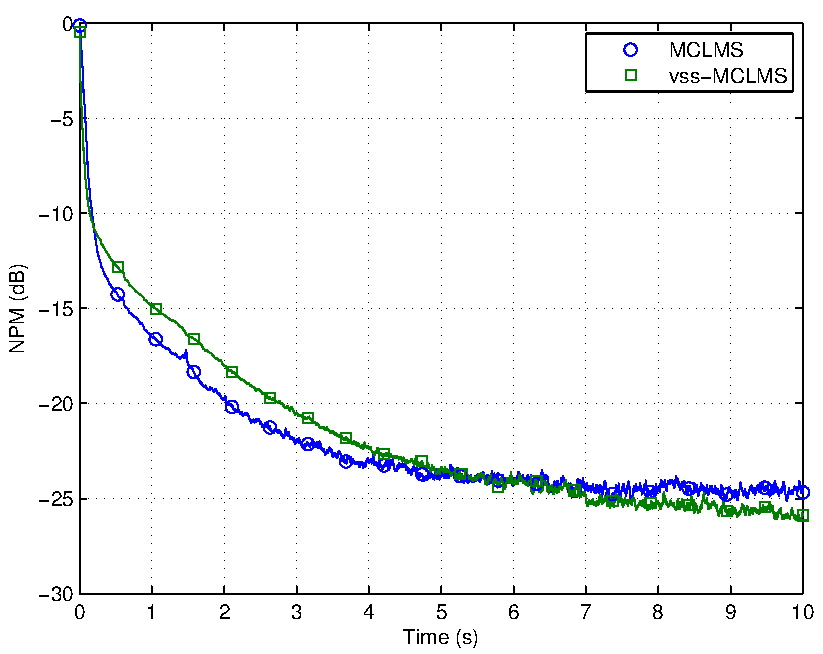
\includegraphics[width=0.475\linewidth]{figs/pdf/mclms_npm.pdf}\label{fig:mclms_npm}} \quad
      \subfigure[Time-domain coefficients of the true and estimated impulse responses of channel $1$ obtained using constrained-MCLMS.]{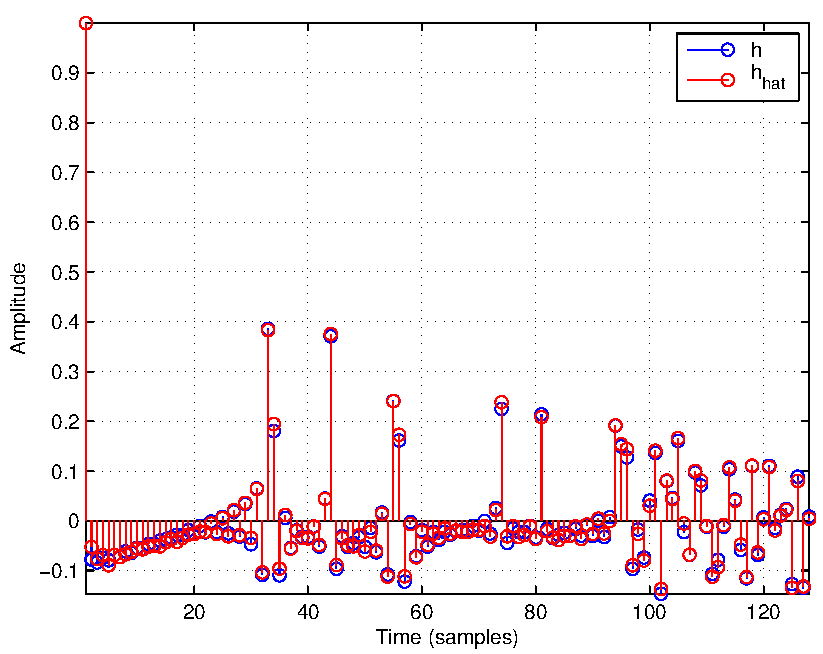
\includegraphics[width=0.475\linewidth]{figs/pdf/mclms_td.pdf} \label{fig:mclms_td}}
      }
      \subfigure[Cost function $J(n)$.]{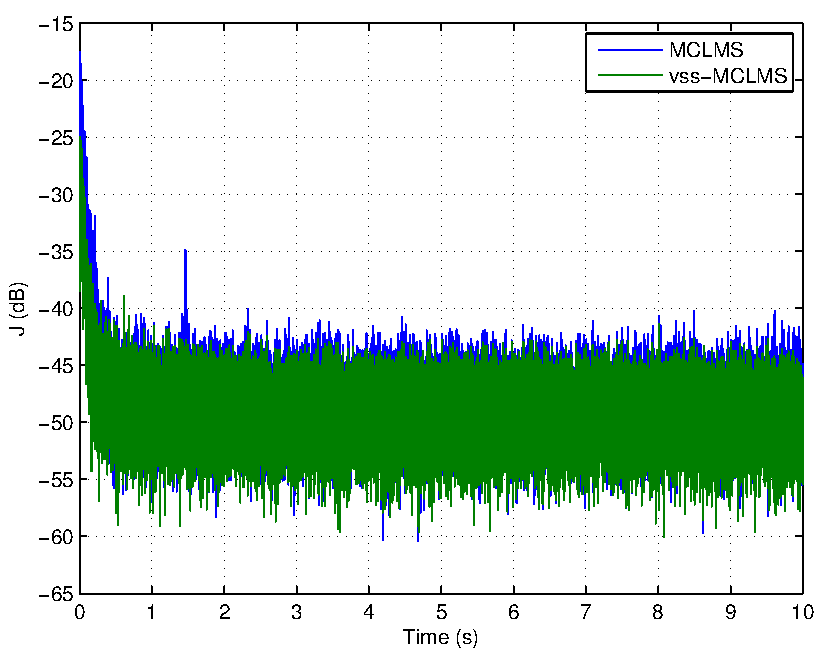
\includegraphics[width=0.475\linewidth]{figs/pdf/mclms_J.pdf}\label{fig:mclms_J}}
    \caption{MCLMS with and without variable step sizes using a WGN source signal (SNR=$30$~dB, $L=128$, $M=5$).}
    \label{fig:mclms}
  \end{center}
\end{figure}

\item[Algorithm] \verb"mclms()" performs the following operations:

\begin{enumerate}[label=\arabic*.]
    %\item Initialize $\mathbf{\widehat{h}}(0)$, where $\widehat{\mathbf{h}}(n)= [\widehat{\mathbf{h}}_1^T(n),~\widehat{\mathbf{h}}_2^T(n),~\ldots,~\widehat{\mathbf{h}}_M^T(n)]^T$.
    \item Computes the CR error at discrete time $n$ using (\ref{eqn:a priori error signal}) and~(\ref{eqn:total a priori error signal}).
    \item Computes the cost function at discrete time $n$ using (\ref{eqn:mclms cost function}).
    \item Computes the instantaneous estimate of the matrix $\mathbf{R}$ given by (\ref{eqn:corrmatrix}).
    \item Updates the adaptive filter coefficients using~(\ref{eqn:mclms_upd2}).
\end{enumerate}
	
\item[Remarks] The MCLMS algorithm is one of the first adaptive blind system identification algorithms proposed in the context of acoustic signal processing. However, it has following limitations:

\begin{itemize}
  \item Slow convergence due to large number of adaptive filter coefficients and the potential presence of common zeros \cite{Lin2006}.
  \item Very sensitive to additive noise \cite{Hasan2006, Gaubitch2006b}.
  \item Does not support complex data and impulse responses.
  \item Smaller step size is preferable for speech input data, but at the cost of slower rate of convergence.
\end{itemize}

\item[See also] \verb"mcn()"
\end{enumerate}

% Multichannel Newton algorithm
\subsection{Multichannel Newton algorithm:~mcn()}

\begin{enumerate}[font=\bf, labelindent=\parindent, widest=123456789012, leftmargin=*, align=left]
	\item[Purpose] Time-domain multichannel Newton adaptive filtering algorithm for blind system identification.
	
	\item[Syntax] \verb"[xin, h_hat, Rhat] = init_mcn(L, N, M, xin0, h_hat0)"

The input and output parameters of \verb"init_mcn()"  are summarized below.

\vspace{-.5em}\begin{verbatim}
Input Parameters [size]:
       L      : filter length
       M      : number of channels
       xin0   : initial input matrix [L x M]
       h_hat0 : initial filter coef. matrix (unit-norm
                constrained) [L x M]

   Output parameters [size]:
       xin    : initialized input matrix [L x M]
       h_hat  : initialized filter coef. matrix [L x M]
       Rhat   : covariance matrix [M L x M L]
\end{verbatim}
	
	\verb"[h_hat, R_hat, J] = mcn(xin, h_hat, R_hat, rho, lambda)" 

The input and output parameters of \verb"mcn()" for an FIR adaptive filter of $L$ coefficients are summarized below.

\vspace{-.5em}\begin{verbatim}
Input parameters:
   	xin   : input matrix [L x M]
       h_hat : current filter coef. matrix [L x M]
       R_hat : covariance matrix [M L x M L]
       rho   : step size (optional: default rho=0.95)
       lamda : exponential forgetting factor (0 < lamda < 1)
               (optional: default lamda=0.99)

Outputs parameters:
       h_hat : updated filter coef. matrix [L x M]
       R_hat : covariance matrix [M L x M L]
       J     : value of cost function
\end{verbatim}

	\item[Description] While the MCLMS algorithm with unit-norm constraint can converge in the mean to the desired channel impulse responses the main difficulty is the selection of the step size $\mu$. As pointed out in many studies, there is a trade-off between the amount of excess mean-squared error, the rate of convergence, and the ability of the algorithm to track changes in the system. In order to obtain a good balance of these competing design objectives, the unit-norm-constrained multichannel Newton algorithm with a variable step size during adaptation was derived in \cite{Huang2002}. The update of the estimated impulse responses is given by:
\begin{equation}\label{eqn:mcn_upd}
	 \mathbf{\widehat{h}}(n) = \mathbf{\widehat{h}}(n-1)-\mathrm{E}^{-1}\{\nabla^2 J(n)\} \, \nabla J(n),
\end{equation}
where $\nabla^2 J(n)$ is the Hessian matrix of $J(n)$ with respect to $\mathbf{\widehat{h}}(n-1)$. With some approximations the unit-norm-constrained update equation can be written as
\begin{equation}\label{eqn:mcn_upd2}
   \mathbf{\widehat{h}}(n) \, = \, \dfrac{\mathbf{\widehat{h}}(n-1)-2\rho\mathbf{V}^{-1}(n)[\widehat{\mathbf{R}}(n)\mathbf{\widehat{h}}(n-1)-E(n)\mathbf{\widehat{h}}(n-1)]}{\left\|\mathbf{\widehat{h}}(n-1)-2\rho\mathbf{V}^{-1}(n)[\widehat{\mathbf{R}}(n)\mathbf{\widehat{h}}(n-1)-E(n)\mathbf{\widehat{h}}(n-1)]\right\|_2},
\end{equation}
where 
\begin{equation} \label{eqn:est mean Hessian}
	\mathbf{V}(n) = 2 \widehat{\mathbf{R}}(n) - 4 \widehat{\mathbf{h}}(n-1) \widehat{\mathbf{h}}^T(n-1) \widehat{\mathbf{R}}(n) - 4 \widehat{\mathbf{R}}(n) \widehat{\mathbf{h}}(n-1) \widehat{\mathbf{h}}^T(n-1)
\end{equation}
approximates $\mathrm{E}\{\nabla^2 J(n)\}$, $\rho$ ($0 < \rho < 1$) denotes the step size that is commonly chosen close to $1$, and $\widehat{\mathbf{R}}(n)$ is an estimate of (\ref{eqn:corrmatrix}) computed using
\begin{equation} \label{eqn:est corrmatrix}
	\widehat{\mathbf{R}}(n) = \lambda \, \widehat{\mathbf{R}}(n-1) + (1-\lambda) \, \widetilde{\mathbf{R}}(n),
\end{equation}
where $\lambda$ ($0 < \lambda < 1$) is an exponential forgetting factor.

	\item[Example] The following is an example script (\verb"test_mcn.m") of running \verb"mcn()" in the context of multi-channel blind system identi�cation. \lstinputlisting{../test/test_mcn.m}
	
	Running the above script (\verb"test_mcn.m") will produce Fig.~\ref{fig:mcn}. Fig.~\ref{fig:mcn_npm} shows the rate of convergence of MCN algorithm in NPM against time. Fig.~\ref{fig:mcn_td} then plots the time-domain samples of $\mathbf{h}_1(n)$ and $\mathbf{\widehat{h}}_1(n)$, where the blue lines indicate the amplitude of each sample of $\mathbf{h}_1(n)$ and the red lines indicate those of $\mathbf{\widehat{h}}_1(n)$. In order to show the estimation performance, the arbitrary scale factor resultant from using MCN algorithm is removed by normalizing the impulse responses in the time domain. Compared to the MNCLMS algorithm the MCN algorithm converges much faster.
\begin{figure}[htbp]
  \begin{center}
    \mbox{
      \subfigure[NPM as a function of time.]{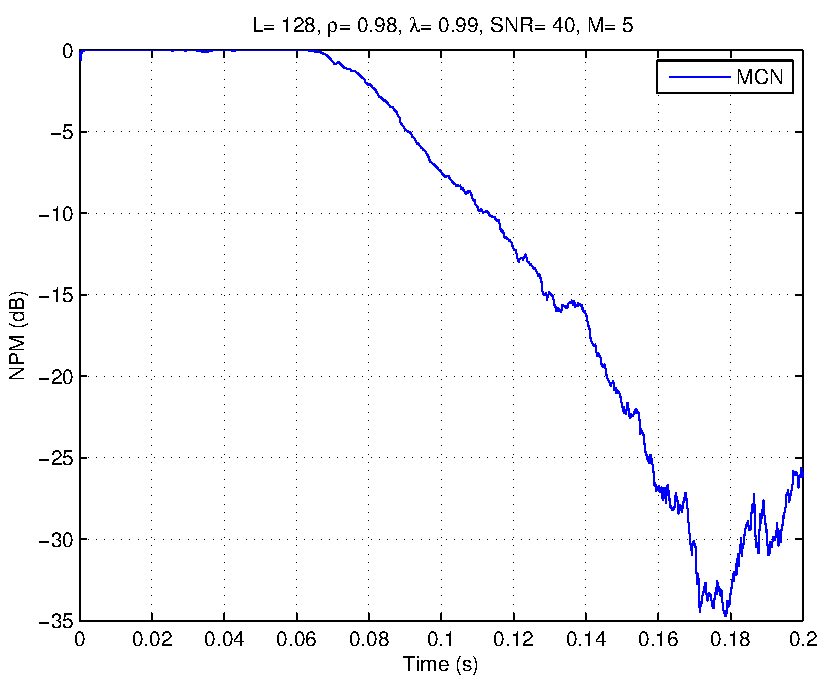
\includegraphics[width=0.475\linewidth]{figs/pdf/mcn_npm.pdf}\label{fig:mcn_npm}} \quad
      \subfigure[Time-domain coefficients of the true and estimated impulse responses of channel $1$.]{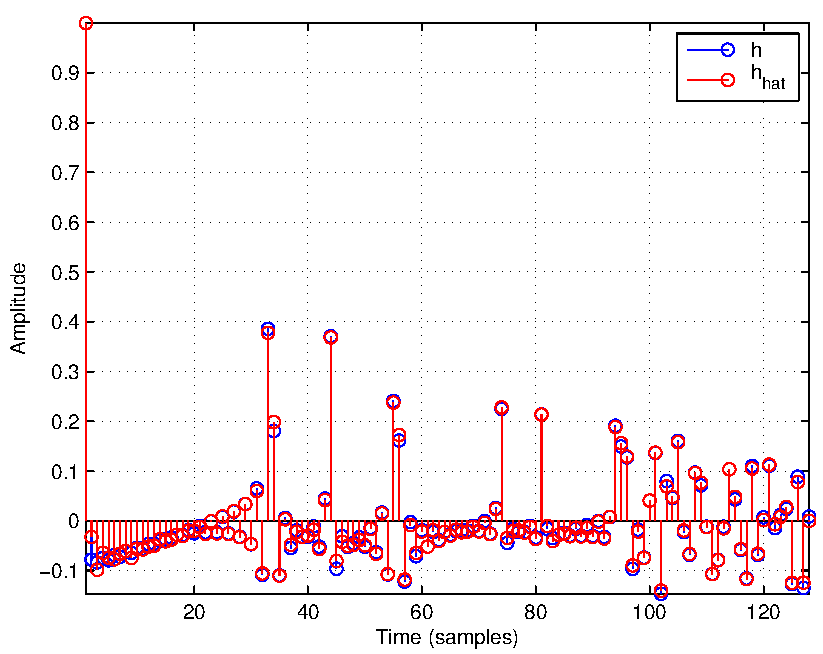
\includegraphics[width=0.475\linewidth]{figs/pdf/mcn_td.pdf} \label{fig:mcn_td}}
      }
    \caption{MCN with WGN source signal (SNR=$40$~dB, $L=128$, $M=5$).}
    \label{fig:mcn}
  \end{center}
\end{figure}

	\item[Algorithm] \verb"mcn()" performs the following operations:
\begin{enumerate}[label=\arabic*.]
%    \item Initialize $\mathbf{\widehat{h}}(0)$, where $\widehat{\mathbf{h}}(n)= [\widehat{\mathbf{h}}_1^T(n),~\widehat{\mathbf{h}}_2^T(n),~\ldots,~\widehat{\mathbf{h}}_M^T(n)]^T$.
    \item Computes the CR error at discrete time $n$ using (\ref{eqn:a priori error signal}) and ~(\ref{eqn:total a priori error signal}).
    \item Computes the cost function at discrete time $n$ using (\ref{eqn:mclms cost function}).
    \item Estimates the matrix $\mathbf{R}$ given by (\ref{eqn:corrmatrix}) using (\ref{eqn:est corrmatrix}).
    \item Updates the adaptive filter coefficients using (\ref{eqn:est mean Hessian}) and~(\ref{eqn:mcn_upd2}).
\end{enumerate}
	
	\item[See also] \verb"mclms()"		
\end{enumerate}

% Multichannel frequency-domain LMS algorithm
\subsection{Multichannel frequency-domain LMS algorithm:~mcflms()}

\begin{enumerate}[font=\bf, labelindent=\parindent, widest=123456789012, leftmargin=*, align=left]
	\item[Purpose] Frequency-domain multichannel LMS adaptive filtering algorithm for blind system identification.
	 	
	\item[Syntax] \verb"[h_hat] = init_mcflms(L, M, h_hat0)"

The input and output parameters of \verb"init_mcflms()" for an FIR adaptive filter of $L$ coefficients are summarized below.

\vspace{-.5em}\begin{verbatim}
Input Parameters [size]:
       L       : filter length
       M       : number of channels
       h_hat0  : initial filter coef. vector 
                 (unit-norm constrained) [L x M]

Output parameters [size]:
       h_hat   : initialized filter coef. matrix [L x M]
\end{verbatim}

 \verb"[h_hat, J] = mcflms(xm, h_hat, mu, ss_cntr)"

The input and output parameters of \verb"mcflms()" for an FIR adaptive filter of $L$ coefficients are summarized below.

\vspace{-.5em}\begin{verbatim}
Input Parameters [size]:
       xm      : input matrix [F x M]
       h_hat   : current filter coef. matrix [L x M]
       mu      : step size (optional: default mu=0.9)
       ss_cntr : type of step-size control 
                 (optional: default `fixed'):
                 `fixed' - fixed with unit-norm-constrained;
                 `vss' - variable step-size
                 `rvss' - robust variable step-size

Output Parameters:
       h_hat   : updated filter coef. matrix [L x M]
       J       : value of the cost function
\end{verbatim}

	\item[Description]
The MCFLMS algorithm is developed based on the derivation of cross-relation~(CR) in the frequency domain. The linear convolution between the $m$th channel output $\mathbf{x}_m(n)$ and the $l$th channel estimate $\mathbf{\widehat{h}}_l(n)$ can be implemented using a vector of length $F=2L$ from the circular convolution
\begin{equation}
    \mathbf{\widetilde{y}}_{ml}(k) \, = \, \mathbf{C}_{x_m}(k)\mathbf{\widehat{h}}^{10}_l(k),
\end{equation}
where $k$ is the frame index, $\mathbf{\widehat{h}}^{10}_l(k)=[\mathbf{\widehat{h}}_l^T(k)~\mathbf{0}^T_{L\times1}]^T$ is the $l$th channel estimate with zero padding, and
\begin{equation}
  \mathbf{C}_{x_m}(k) = \left[%
  \begin{array}{cccc}
  x_m(kL-L) & x_m(kL+L-1) & \cdots & x_m(kL-L+1) \\
  x_m(kL-L+1) & x_m(kL-L) & \cdots & x_m(kL-L+2) \\
  \vdots & \vdots & \ddots & \vdots \\
  x_m(kL+L-1) & x_m(kL+L-2) & \cdots & x_m(kL-L) \\
  \end{array}%
  \right]
\end{equation}
is the $2L\times2L$ circulant matrix constructed from
\begin{equation}
    \boldsymbol{\chi}_m(k) \, = \, [x_m(kL-L)~x_m(kL-L+1)~\ldots~x_m(kL+L-1)]^T.
\end{equation}
It should be noted that $\mathbf{C}_{x_m}(k)$ is only determined by $\boldsymbol{\chi}_m(k)$, e.g., the second column of $\mathbf{C}_{x_m}(k)$ is the shifted version of $\boldsymbol{\chi}_m(k)$. A $50\%$ overlap-save\footnote{It should be noted that the implementation allows the use of any overlap smaller or equal than $50\%$. However, the most computational efficient implementation is obtained with $50\%$ overlap.} is employed so that $L$ previous samples of $\mathbf{x}_m(n)$ are included in $\boldsymbol{\chi}_m(k)$. For each $\mathbf{\widetilde{y}}_{ml}(k)$ of length $2L$, the last $L$ samples are retained since they correspond to the linear convolution given by $\mathbf{x}_m^T(n)\mathbf{\widehat{h}}_l(n)$. As a result, by defining two selecting matrices
\begin{equation}
    \mathbf{W}_{L\times 2L}^{01} \, = \, [\mathbf{0}_{L\times L}~\mathbf{I}_{L\times L}], \qquad
  \mathbf{W}_{2L\times L}^{10} \, = \, [\mathbf{I}_{L\times L}~\mathbf{0}_{L\times L}]^T
\end{equation}
the desired result $\mathbf{y}_{ml}(k)$ can be obtained 
\begin{align}
    \mathbf{y}_{ml}(k) & =  \mathbf{W}_{L\times 2L}^{01}\mathbf{\widetilde{y}}_{ml}(k) \, = \,
    \mathbf{W}_{L\times 2L}^{01}\mathbf{C}_{x_m}(k)\mathbf{\widehat{h}}^{10}_l(k), \nonumber \\
    & =  \mathbf{W}_{L\times 2L}^{01}\mathbf{C}_{x_m}(k)\mathbf{W}_{2L\times L}^{10}\mathbf{\widehat{h}}_l(k).
\end{align}
To employ FFT techniques for efficient implementation of circular convolution, it is important to note that the circulant matrix $\mathbf{C}_{x_m}(k)$ can be decomposed as
\begin{equation}
    \mathbf{C}_{x_m}(k) \, = \, \mathbf{F}^{-1}_{2L}\boldsymbol{\underline{\mathcal{D}}}_m(k)\mathbf{F}_{2L},
\end{equation}
where $\mathbf{F}_{2L}$ is a $2L\times2L$ DFT matrix with $\mathbf{F}^{-1}_{2L}=\mathbf{F}^H_{2L}/(2L)$, and $\boldsymbol{\underline{\mathcal{D}}}_m(k)$ is a diagonal matrix with diagonal elements being given by the DFT of $\boldsymbol{\chi}_m(k)$. Now, the frequency-domain CR error function can be written
\begin{align}
  \boldsymbol{\underline{e}}_{ml}(k) &= \mathbf{F}_{L}\left[\mathbf{y}_{ml}(k)-\mathbf{y}_{lm}(k)\right], \nonumber\\
   &= \mathbf{F}_{L}\mathbf{W}_{L\times 2L}^{01}\left[\mathbf{C}_{x_m}(k)\mathbf{W}_{2L\times L}^{10}\mathbf{\widehat{h}}_l(k)-
   \mathbf{C}_{x_l}(k)\mathbf{W}_{2L\times L}^{10}\mathbf{\widehat{h}}_m(k)\right], \nonumber\\
   &= \boldsymbol{\mathcal{W}}_{L\times 2L}^{01}\left[\boldsymbol{\underline{\mathcal{D}}}_m(k)\boldsymbol{\mathcal{W}}^{10}_{2L\times L}
   \underline{\mathbf{\widehat{h}}}_l(k)-\boldsymbol{\underline{\mathcal{D}}}_l(k)\boldsymbol{\mathcal{W}}^{10}_{2L\times L}
   \underline{\mathbf{\widehat{h}}}_m(k)\right], \label{eqn:FD CR error}
\end{align}
for $m,l=1,2,\ldots,M,~m\neq l$, where
\begin{equation}
  \boldsymbol{\mathcal{W}}_{L\times 2L}^{01} \, = \, \mathbf{F}_{L}\mathbf{W}_{L\times 2L}^{01}\mathbf{F}^{-1}_{2L},~~
  \boldsymbol{\mathcal{W}}^{10}_{2L\times L} \, = \, \mathbf{F}_{2L}\mathbf{W}_{2L\times L}^{10}\mathbf{F}^{-1}_{L},
\end{equation}
\begin{equation}\label{eqn:ch_fsd_hhat_freq}
    \underline{\mathbf{\widehat{h}}}_m(k) \, = \, \mathbf{F}_L\mathbf{\widehat{h}}_m(k).
\end{equation}
The MCFLMS algorithm is therefore given by \cite{Huang2003}, for $m=1,2,\ldots,M$,
\begin{align}
  \boldsymbol{\underline{e}}_{ml}^{01}(k) &= \boldsymbol{\mathcal{W}}_{2L\times L}^{01}
  \boldsymbol{\underline{e}}_{ml}(k)~=~\mathbf{F}_{2L}\left[%
    \begin{array}{c}
    \mathbf{0}_{L\times1} \\
    \mathbf{F}^{-1}_{L}\boldsymbol{\underline{e}}_{ml}(k) \\
    \end{array}%
    \right], \label{eqn:ch_fsd_e_freq01}\\
  \mathbf{\underline{\widehat{h}}}_m^{10}(k-1) &= \mathbf{F}_{2L}\mathbf{\widehat{h}}_m^{10}(k-1)~=~
  \mathbf{F}_{2L}\mathbf{W}_{2L\times L}^{10}\mathbf{\widehat{h}}_m(k-1), \label{eqn:constrain_hhat_freq10}\\    
  \mathbf{\widehat{\underline{h}}}_m^{10}(k) &=
  \mathbf{\widehat{\underline{h}}}_m^{10}(k-1)-\mu \sum^M_{l=1}\boldsymbol{\underline{\mathcal{D}}}^*_l(k)\boldsymbol{\underline{e}}_{ml}^{01}(k) \label{eqn:upd_hhat_freq10}
\end{align}
where $\mu$ is the step size, and
\begin{equation}
    \boldsymbol{\mathcal{W}}_{2L\times L}^{01} \, = \, \mathbf{F}_{2L}\mathbf{W}_{2L\times L}^{01}\mathbf{F}^{-1}_{L} \, = \, 2\left(\boldsymbol{\mathcal{W}}_{L\times 2L}^{01}\right)^H
\end{equation}
with $\mathbf{W}_{2L\times L}^{01}=\left(\mathbf{W}_{L\times 2L}^{01}\right)^T$. To satisfy the unit-norm constraint \cite{Huang2003}, the frequency-domain coefficients of the adaptive filter are initialized as $\mathbf{\widehat{\underline{h}}}_m^{10}(0)=(\mathbf{1}_{2L\times1})/\sqrt{M}$.	

The performance of the MCFLMS algorithm is highly dependent upon the step size. The standard MCFLMS uses a fixed step size. Two alternative variable step sizes are available, viz., \verb"vss" and \verb"rvss", that were derived in \cite{Haque2008}.

\item[Example] The following is an example script (\verb"test_mcflms.m") of running \verb"mcflms()" in the context of multichannel blind system identification.

\lstinputlisting{../test/test_mcflms.m}

Running the above script (\verb"test_mcflms.m") will produce Fig.~\ref{fig:mcflms}. Fig.~\ref{fig:mcflms_npm} showing the rate of convergence of MCFLMS algorithm in NPM against time. Fig.~\ref{fig:mcflms_td} then plots the time-domain samples of $\mathbf{h}_1(n)$ and $\mathbf{\widehat{h}}_1(n)$, where the blue lines indicate the amplitude of each sample of $\mathbf{h}_1(n)$ and the red lines indicate those of $\mathbf{\widehat{h}}_1(n)$. In order to show the estimation performance, the arbitrary scale factor resultant from using MCFLMS algorithm is removed by normalizing the impulse responses in the time domain.
\begin{figure}[htbp]
  \begin{center}
    \mbox{
      \subfigure[NPM as a function of time.]{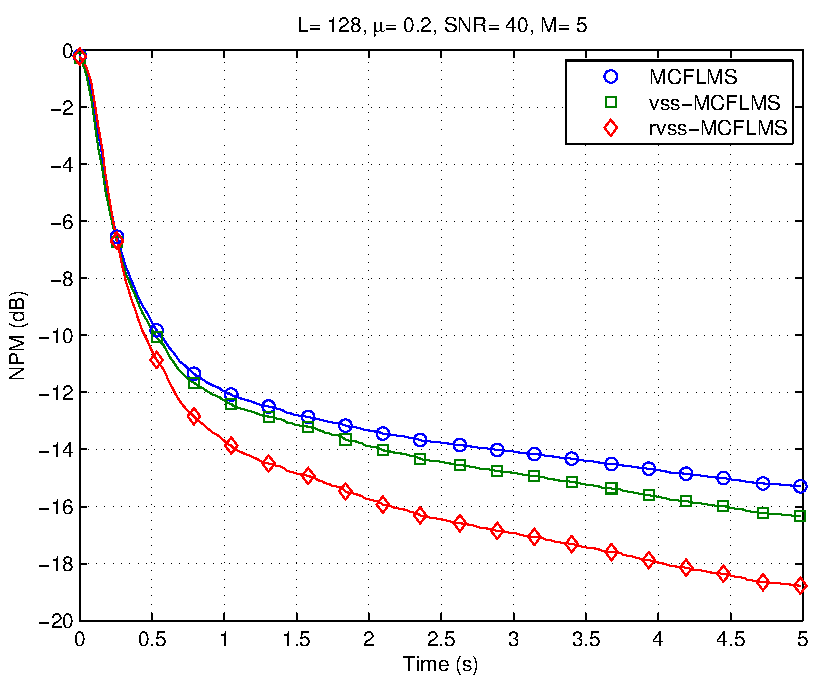
\includegraphics[width=0.475\linewidth]{figs/pdf/mcflms_npm.pdf}\label{fig:mcflms_npm}} \quad
      \subfigure[Time-domain coefficients of the true and estimated impulse responses of channel $1$ obtained using constrained-MCFLMS.]{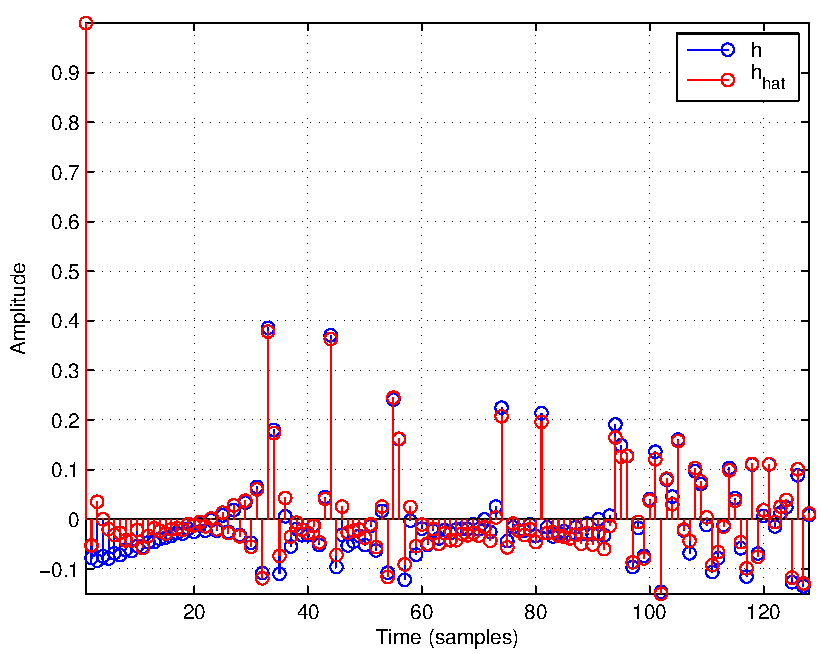
\includegraphics[width=0.475\linewidth]{figs/pdf/mcflms_td.pdf} \label{fig:mcflms_td}}
      }
    \caption{MCFLMS with different step size mechanisms and a WGN source signal (SNR=$40$~dB, $L=128$, $M=5$).}
    \label{fig:mcflms}
  \end{center}
\end{figure}
	
\item[Algorithm] \verb"mcflms()" performs the following operations:

\begin{enumerate}[label=\arabic*.]
    \item Computes the CR error of time frame $k$ using (\ref{eqn:FD CR error}) and (\ref{eqn:ch_fsd_e_freq01}).
    \item Computes the cost function for time frame $k$.
    \item Updates the adaptive filter coefficients using (\ref{eqn:constrain_hhat_freq10}) and (\ref{eqn:upd_hhat_freq10}).
\end{enumerate}
	
	\item[See also] \verb"mclms()", \verb"mcn()", \verb"nmcflms()" 	
\end{enumerate}

% Normalized multichannel frequency-domain LMS algorithm
\subsection{Normalized multichannel frequency-domain LMS algorithm:\\nmcflms()}

\begin{enumerate}[font=\bf, labelindent=\parindent, widest=123456789012, leftmargin=*, align=left]
	\item[Purpose] Normalized Frequency-domain multichannel LMS adaptive filtering algorithm for blind system identification.
	
	\item[Syntax] \verb"[h_hat, P_k] = init_nmcflms(L, F, M, xm0, h_hat0)"

The input and output parameters of \verb"init_nmcflms()" are summarized below.

\vspace{-.5em}\begin{verbatim}
Input Parameters [size]:
       L      : filter length
       F      : frame length
       M      : number of channels
       xm0    : initial input block used 
                to calculate P_k [F x M]
       h_hat0 : initial filter coef. matrix 
                (unit-norm constrained) [L x M]

Output parameters [size]:
       h_hat  : initialized filter coef. matrix [L x M]
       P_k    : initialized PSDs [F x M]
\end{verbatim}

\verb"[h_hat, P_k, J] = nmcflms(xm, h_hat, P_k, ro, lambda, delta)" 

The input and output parameters of \verb"nmcflms()" for an FIR adaptive filter of $L$ coefficients are summarized below.

\vspace{-.5em}\begin{verbatim}
Input Parameters [size]:
       xm      : input matrix [F x M]
       h_hat   : current filter coef. matrix [L x M]
       P_k_avg : estimated PSD matrix [F x M]
       rho     : step size (optional: default rho=0.8)
       lambda  : exponential forgetting factor 
                 (0 < lambda < 1) (optional)
       delta   : regularization (optional)

Output Parameters:
       h_hat   : updated filter coef. matrix [L x M]
       P_k_avg : updated PSD matrix [F x M]
       J       : cost function values [F-L+1 x 1]
\end{verbatim}

	\item[Description] 
The NMCFLMS algorithm is given by \cite{Huang2003}, for $m=1,2,\ldots,M$,
\begin{align}
  \boldsymbol{\underline{\mathcal{P}}}_m(k) &= \lambda\boldsymbol{\underline{\mathcal{P}}}_m(k-1)+(1-\lambda)
  \sum^M_{l=1,l\neq m}\boldsymbol{\underline{\mathcal{D}}}^*_l(k)\boldsymbol{\underline{\mathcal{D}}}_l(k), \\
   \mathbf{\widehat{\underline{h}}}_m^{10}(k) &=
  \mathbf{\widehat{\underline{h}}}_m^{10}(k-1)-\mu[\boldsymbol{\underline{\mathcal{P}}}_m(k)+\delta\mathbf{I}_{2L\times 2L}]^{-1}
  \times\sum^M_{l=1}\boldsymbol{\underline{\mathcal{D}}}^*_l(k)\boldsymbol{\underline{e}}_{ml}^{01}(k) \label{eqn:upd_hhat_freq10_with_normalization},
\end{align}
where $\lambda=[1-1/(3L)]^L$ is the forgetting factor, $\mu$ is the step size, $\delta$ is the regularization parameter. To satisfy the unit-norm constraint \cite{Huang2003}, the frequency-domain coefficients of the adaptive filter are initialized as $\mathbf{\widehat{\underline{h}}}_m^{10}(0)=(\mathbf{1}_{2L\times1})/\sqrt{M}$.

In addition to the standard NMCFLMS algorithm the toolbox also facilitates the robust NMCFLMS (RNMCFLMS) algorithm (\verb"rnmcflms()") derived in \cite{Haque2008}, for details regarding this algorithm we refer the reader to that publication.
	
	\item[Example] Here we present two example scripts that use \verb"nmcflms()" and \verb"rnmcflms()" in the context of multi-channel blind system identi�cation. The first example script (\verb"test_nmcflms.m") uses a WGN source signal: \lstinputlisting{../test/test_nmcflms.m}
	
Running the above script (\verb"test_nmcflms.m") will produce Fig.~\ref{fig:nmcflms}. Fig.~\ref{fig:nmcflms_npm} shows the rate of convergence of NMCFLMS algorithm in NPM against time. Fig.~\ref{fig:nmcflms_td} then plots the time-domain samples of $\mathbf{h}_1(n)$ and $\mathbf{\widehat{h}}_1(n)$, where the blue lines indicate the amplitude of each sample of $\mathbf{h}_1(n)$ and the red lines indicate those of $\mathbf{\widehat{h}}_1(n)$. In order to show the estimation performance, the arbitrary scale factor resultant from using NMCFLMS algorithm is removed by normalizing the impulse responses in the time domain.
\begin{figure}[htbp]
  \begin{center}
    \mbox{
      \subfigure[NPM as a function of time.]{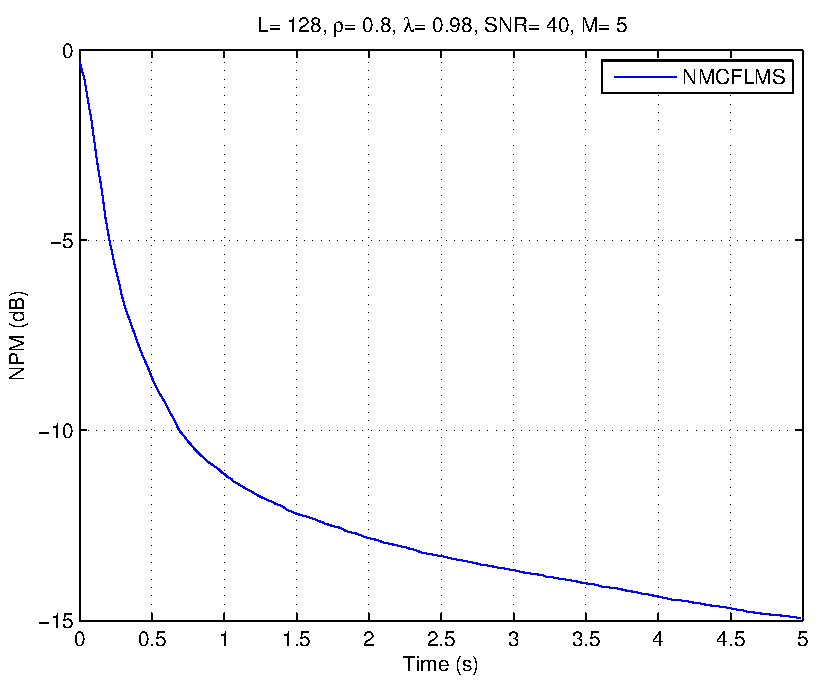
\includegraphics[width=0.475\linewidth]{figs/pdf/nmcflms_npm.pdf}\label{fig:nmcflms_npm}} \quad
      \subfigure[Time-domain coefficients of the true and estimated impulse responses of channel $1$.]{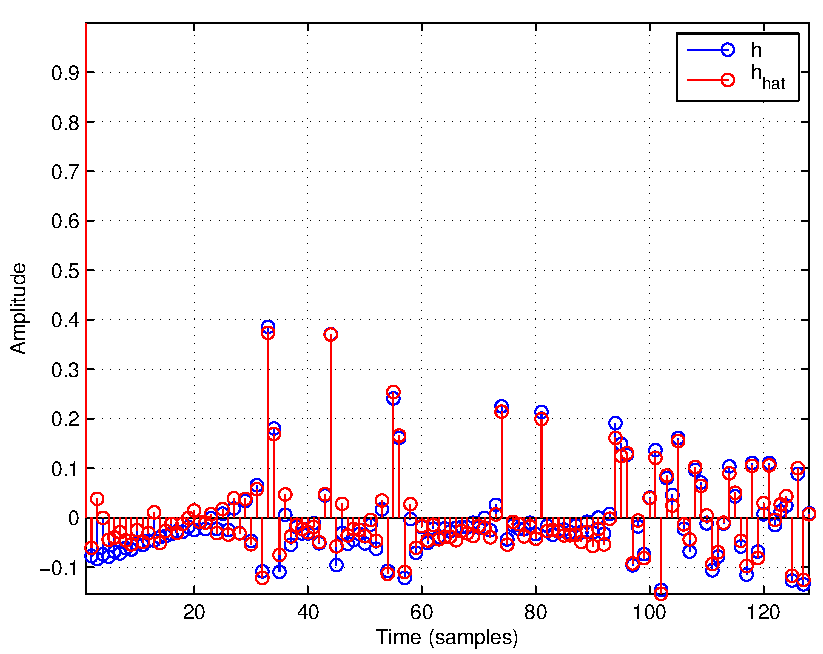
\includegraphics[width=0.475\linewidth]{figs/pdf/nmcflms_td.pdf} \label{fig:nmcflms_td}}
      }
    \caption{NMCFLMS with WGN source signal (SNR=$40$~dB, $L=128$, $M=5$).}
    \label{fig:nmcflms}
  \end{center}
\end{figure}

The second example script (\verb"test_rnmcflms_speech.m") uses a male speech source signal:

\lstinputlisting{../test/test_rnmcflms_speech.m}
	
Running the above script (\verb"test_rnmcflms_speech.m") will produce four figures as shown in Fig.~\ref{fig:nmcflms_speech}.  Fig.~\ref{fig:nmcflms_speech_mic} shows the signal received by the first microphone. Fig.~\ref{fig:nmcflms_speech_npm} shows the rate of convergence of RNMCFLMS algorithm in NPM against time. Fig.~\ref{fig:nmcflms_speech_td} then plots the time-domain samples of $\mathbf{h}_1(n)$ and $\mathbf{\widehat{h}}_1(n)$, where the blue lines indicate the amplitude of each sample of $\mathbf{h}_1(n)$ and the red lines indicate those of $\mathbf{\widehat{h}}_1(n)$. Fig.~\ref{fig:nmcflms_speech_fd} shows the magnitude response of the true and estimate impulse responses of the first acoustic channel.
\begin{figure}[htbp]
  \begin{center}
    \mbox{
      \subfigure[Reverberant signal received by the first microphone.]{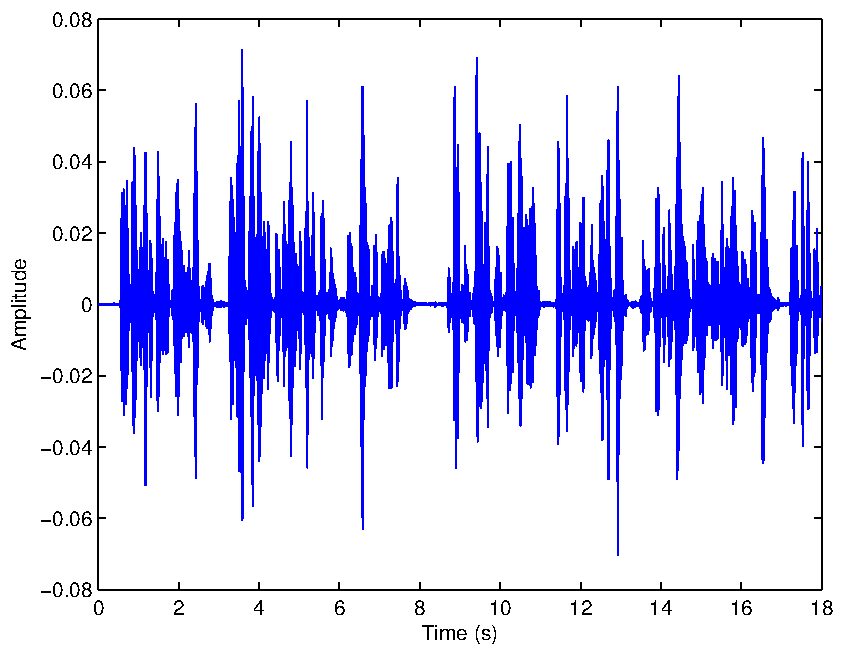
\includegraphics[width=0.475\linewidth]{figs/pdf/nmcflms_speech_mic.pdf}\label{fig:nmcflms_speech_mic}} \quad
      \subfigure[NPM as a function of time.]{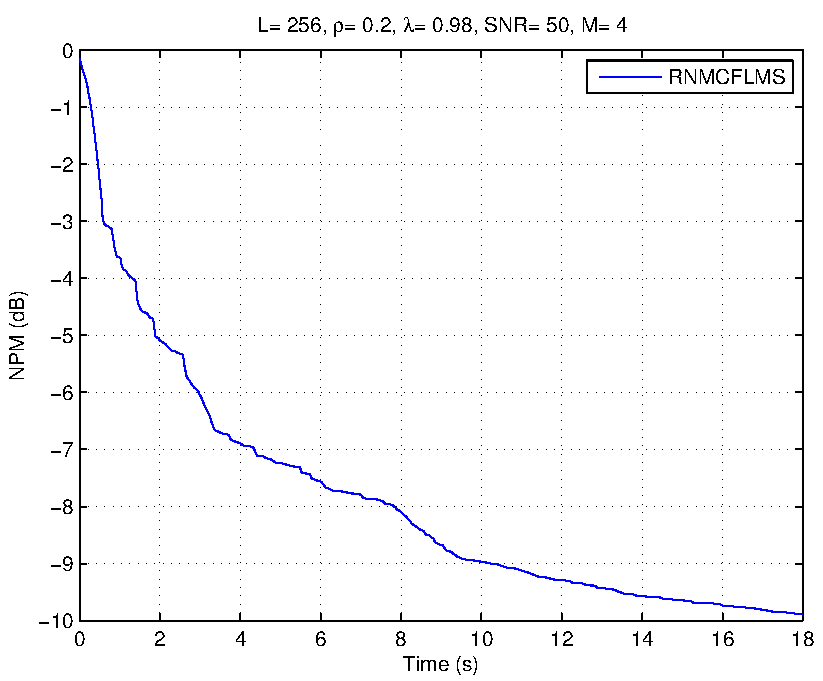
\includegraphics[width=0.475\linewidth]{figs/pdf/nmcflms_speech_npm.pdf} \label{fig:nmcflms_speech_npm}}
      }
    \mbox{
      \subfigure[Time-domain coefficients of the true and estimated impulse responses of channel $1$.]{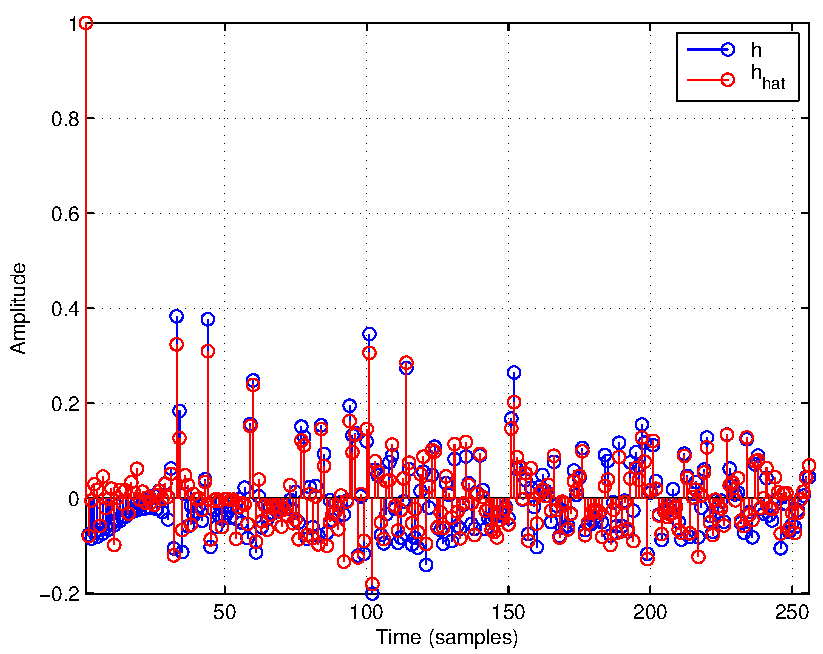
\includegraphics[width=0.475\linewidth]{figs/pdf/nmcflms_speech_td.pdf}\label{fig:nmcflms_speech_td}} \quad
      \subfigure[Magnitude response of the true and estimated impulse responses of channel $1$.]{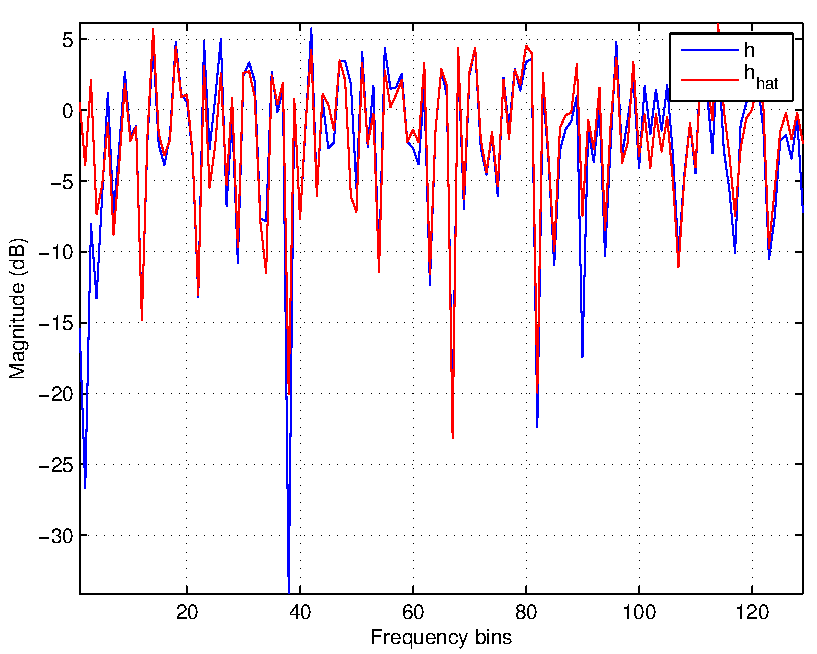
\includegraphics[width=0.475\linewidth]{figs/pdf/nmcflms_speech_fd.pdf}\label{fig:nmcflms_speech_fd}} 
      }
    \caption{RNMCFLMS with speech source signal (SNR = $50$~dB, $L=256$, $M=4$).}
    \label{fig:nmcflms_speech}
  \end{center}
\end{figure}

	\item[Algorithm]  \verb"nmcflms()" performs the following operations:

\begin{enumerate}[label=\arabic*.]
    \item Computes the CR error of time frame $k$ using (\ref{eqn:FD CR error}) and (\ref{eqn:ch_fsd_e_freq01}).
    \item Computes the cost function for time frame $k$.
    \item Updates the adaptive filter coefficients using~(\ref{eqn:upd_hhat_freq10_with_normalization}) and (\ref{eqn:constrain_hhat_freq10}).
\end{enumerate}
	
	\item[See also] \verb"mclms()", \verb"mcn()", \verb"mcflms()" 		
\end{enumerate}

% Normalized Multichannel Multi-Delay Filter LMS Algorithm
\subsection{Normalized Multichannel Multi-Delay Filter LMS Algorithm:\\nmcmdflms()}

\begin{enumerate}[font=\bf, labelindent=\parindent, widest=123456789012, leftmargin=*, align=left]
	\item[Purpose] Normalized Frequency-domain multichannel multi-delay filtering LMS adaptive filtering algorithm for blind system identification.
	
	\item[Syntax] \verb"[shMDF, H_hat] = init_nmcmlflms(L, Ms, Mch, xm0, H_hat0)"

The input and output parameters of \verb"init_nmcmdflms()" are summarized below.

\vspace{-.5em}\begin{verbatim}
Input Parameters [size]:
       L      : filter length
       Ms     : number of MDF channels
       Mch    : number of channels
       xm0    : input data
       H_hat0 : initial filter coef. matrix 
       	 	      (unit-norm constrained) [L x M]

Output parameters [size]:
       shMDF  : MDF data structure
       H_hat  : initialized filter coef. matrix [L x M]
\end{verbatim}

The input and output parameters of \verb"nmcmdflms()" for an FIR adaptive filter of $L$ coefficients are summarized below.

\verb"[shMDF H_hat J] = nmcmdflms(shMDF, xm, rho, lambda, delta)" 

\vspace{-.5em}\begin{verbatim}
   Input Parameters [size]:
       shMDF    : MDF structure
       xm       : input matrix [F x M]
       H_hat    : current filter coef. matrix [L x M]
       rho      : step size (optional: default rho=0.2)
       lambda   : exponential forgetting factor (0 < lambda < 1) (optional)
       delta    : regularization (optional)

   Output Parameters:
       shMDF    : MDF structure
       H_hat    : updated filter coef. matrix [L x M]
       J        : cross-relation error [Ms x Mch x Mch]
 
   shMDF structure:
       H_hat    : MDF representation of H_hat (MC)
       Xm       : MDF representation of x - with overlapping (MC)
       Ms       : number of MDF segments (blocks).
       Mch      : number of channels
       Nm       : segment length
\end{verbatim}

\item[Description] 
The NMCMDFLMS algorithm is found in~\cite{Ahmad2006a}. The MDF structure~\cite{Soo1990} reduces the problem of delay in frequency domain algorithm implementation by partitioning the adaptive filter of length $L$ into $K$ blocks such that $L=KN$ where $N$ is the block length. Let $m$ be the frame index and we define input matrix $\mathbf{X}_i(m)$ and \emph{a priori} error $\mathbf{e}_{ij}(m)$ for $i\neq j$:
\begin{align}
	\X_i(m)&=[\x_i(mN)\dots \x_i(nM+N-1)],~i=1,2,\dots,M,\\
	\e_{ij}(m)&=\X_i(m)\hh_j(m-1)-\X_j(m)\hh_i(m-1)\\
			&=[e_{ij}(mN)\dots e_{ij}(mN+N-1)]^T.
\end{align}
Defining $k$ as the block index, the diagonal data matrix $\D_{x_i}(m)$ for channel $i$ is
\begin{align}
	\D_{x_i}(m)&=\mathrm{diag}\{\F_{2N}\boldsymbol{\chi}_i(m)\},\\
	\boldsymbol{\chi}_i(m)&=[x_i(\tau+N)~x_i(\tau-N+1)\dots x_i(\tau+N-1)]^T,
\end{align}
where $\tau=mN-kN$. Note that the first element of the diagonal of $\D_{x_i}(m)$ is arbitrary, but it is normally equal to the first sample of the previous block $k-1$~\cite{Benesty2001}. We now define the frequency domain quantities: $\underline{\hh}_{i,k}(m)=\F_{2N} \left[ \begin{array}{c}
    \hh_{i,k}(m) \\
    \mathbf{0}_{N \times 1}\\
    \end{array}\right]$,
$\underline{\e}_{i,j}(m)=\F_{2N} \left[ \begin{array}{c}
    \mathbf{0}_{N \times 1} \\
    \e_{i,j}(m) \\
    \end{array}\right]$,
$\W^{01}_{2N \times 2N}=\left[ \begin{array}{cc}
    \mathbf{0}_{N \times N} & \mathbf{0}_{N \times N} \\
    \mathbf{0}_{N \times N} & \I_{N \times N}\\
    \end{array}\right]$,
$\W^{10}_{2N \times 2N}=\left[ \begin{array}{cc}
    \I_{N \times N} & \mathbf{0}_{N \times N} \\
    \mathbf{0}_{N \times N} & \mathbf{0}_{N \times N}\\
    \end{array}\right]$,
$\G^{10}_{2N \times 2N}=\F_{2N}\W^{10}_{2N \times 2N}\F^{-1}_{2N}$ and $\G^{01}_{2N \times 2N}=\F_{2N}\W^{01}_{2N \times 2N}\F^{-1}_{2N}$, where $\underline{\hh}_{i,k}(m)$ is the $k^{\mathrm{th}}$ subfilter of the $i^{\mathrm{th}}$ channel, for $k=0,\dots,K-1$ and $i=1,\dots,M$. The MCMDF adaptive algorithm for BCI is then given by
\begin{align}
	\underline{\e}_{ij}(m)=&\G^{01}_{2N \times 2N}\sum_{k=0}^{K-1}\D_{x_i}(m-k)\underline{\hh}_{j,k}(m-1)-\\
					  &\G^{01}_{2N \times 2N}\sum_{k=0}^{K-1}\D_{x_j}(m-k)\underline{\hh}_{i,k}(m-1),\\
	\S_i(m) 			=&\lambda \S_i(m-1)+\\
					 &(1-\lambda)\sum_{j=1,j\neq i}^M \D^\ast_{x_j}(m)\D_{x_j}(m),\\
	\underline{\hh}_{i,k}(m)=&\underline{\hh}_{i,k}(m-1)-\beta \G^{10}_{2N \times 2N} \times \\
					       &[\S_i(m)+\delta_{\textrm{MDF}}]^{-1}\sum_{j=1}^M\D^\ast_{x_j}(m-k)\underline{\e}_{ji}(m),
\end{align}
where $\beta$ is the step size $0 \ll \lambda < 1$ is the forgetting factor. Defining $\sigma^2_x$ as the input signal variance, $\S_i(0)=\sigma_{x_i}^2/100$ is the initialization~\cite{Benesty2001} and $\delta_{\mathrm{MDF}}$ is the regularization constant which is set to one fifth the total power over all channels at the first frame~\cite{Huang2003}.

\item[Example] Here we present an example script that uses \verb"nmcmdflms()" in the context of multi-channel blind system identi�cation. The example script (\verb"test_nmcdfflms.m") uses a WGN source signal: \lstinputlisting{../test/test_nmcmdflms.m}

Running the above script (\verb"test_nmcmdflms.m") will produce Fig.~\ref{fig:nmcmdflms}, showing the rate of convergence of NMCMDFLMS algorithm in NPM against time. 

\begin{figure}[!h]
\centerline{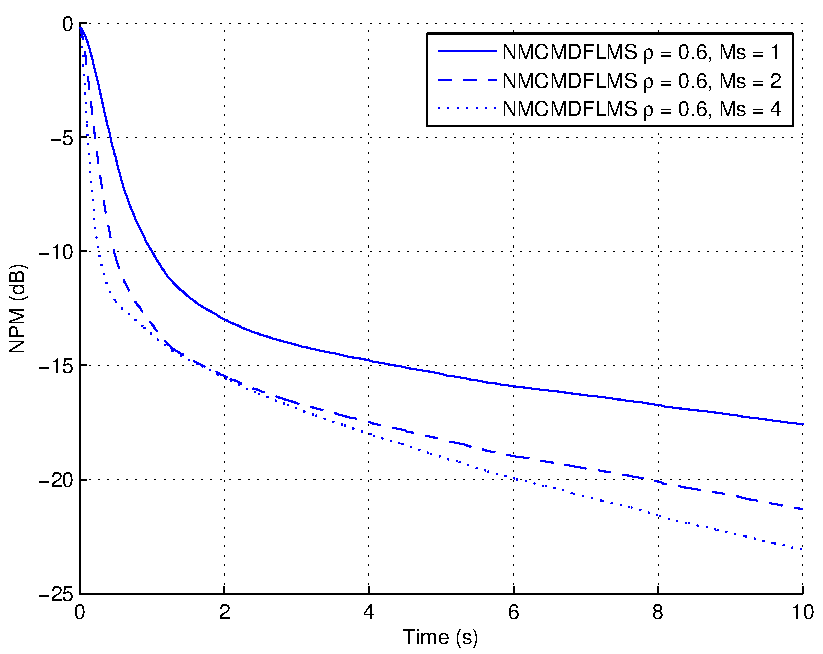
\includegraphics[width=0.5\columnwidth]{figs/pdf/nmcmdflms.pdf}}
 \caption{NMCMDFLMS with WGN source signal (SNR=$40$~dB, $L=128$, $M=5$).}
\label{fig:nmcmdflms}
\end{figure}


\end{enumerate}

%
% System Equalization
%
\section{System Equalization}
In this Section various algorithms are describe that compute a set of equalization filters given the estimated impulse responses of the acoustic system.

% Introduction

% Least squares algorithm
\subsection{Least squares algorithm:~lsinvfilt()}

\begin{enumerate}[font=\bf, labelindent=\parindent, widest=123456789012, leftmargin=*, align=left]
	\item[Purpose] Design a set of equalization filters given the estimated channel impulse responses.
	
	\item[Syntax] \verb"[g] = lsinvfilt(h_hat, Li, k)" 

The input and output parameters of \verb"lsinvfilt()" for an FIR system of size $L \times M$ are summarized below.\vspace{5pt}

\verb"Input Parameters [size]:" \vspace{5pt}

\begin{tabular}[c]{l l l}
  \verb"h_hat" &:& \verb"M impulse responses of length L [L x M]"\\
  \verb"Li" &:& \verb"length of the equalization filters" \\  
  \verb"k" &:& \verb"delay of the target response"\\
\end{tabular}\\
\vspace{5pt}

\verb"Output Parameters [size]:" \vspace{5pt}

\begin{tabular}[c]{l l l}
  \verb"g" &:& \verb"equalization filters [Li x M]" \\
\end{tabular}\\
\vspace{5pt}

%	Input Parameters [size]:
%       h    : M impulse responses of length L [L x M] 
%       Li   : length of the equalization filters
%       k    : delay of the target response
%
%   Output parameters [size]:
%       g    : equalization filters [Li x M] 	
	
	\item[Description] A set of equalization filters, with length $L_i$, can be calculated by solving the following system of equations
\begin{equation}
\sum_{m=1}^M \widehat{h}_m(j)\ast
g_m(j)=d(j)\quad\mbox{for}\;j=0,\ldots,L+L_i-2, \label{eqn:ben}
\end{equation}
where
\begin{equation}
  d(j)=\left\{ \begin{array}{cl}
              0 & \mbox{if}~ 0 \leq j<\tau; \\
              1 & \mbox{if}~ j=\tau; \\
              0 & \mbox{otherwise},
       \end{array} \right.
  \end{equation}
represents the target response with delay $\tau$. In matrix form, (\ref{eqn:ben}) can
be written as
\begin{equation}
\widehat{\H}\g=\d, \label{eqn:be}
\end{equation}
where  $\d=[d(0)\cdots
d(L+L_i-2)]^{T}$ represents the target response vector and 
\begin{equation}
\widehat{\H}=[\widehat{\H}_1~\cdots~\widehat{\H}_M]
\end{equation}
with $\widehat{\H}_m$ an $(L+L_i-1)\times L_i$ convolution matrix of $\widehat{\h}_m$:
\begin{equation}
\widehat{\H}_m= \left[
\begin{array}{cccc}
\widehat{h}_m(0) & 0 & \cdots & 0\\
\widehat{h}_m(1) & \widehat{h}_m(0) & \cdots & 0\\
\vdots & \ddots & \ddots & \vdots\\
\widehat{h}_m(L-1) & \cdots & \vdots & \vdots\\
0 & \widehat{h}_m(L-1) & \ddots & \vdots\\
\vdots & \vdots & \ddots & \vdots\\
0 & \ldots & 0 & \widehat{h}_m(L-1)
\end{array} \right].
\end{equation}
For single channel case, where $M=1$, (\ref{eqn:be}) is always an over-determined system of equations. The LS solution that minimizes the cost function
\begin{equation}
J=\|\widehat{\H}\g-\d\|_2^2, \label{eqn:csf},
\end{equation}
has been used for acoustic system equalization \cite{Mourjopoulos1982}. The LS solution is given by
\begin{equation}
\g=\widehat{\H}^\dag \d, \label{eqn:gls}
\end{equation}
where $\{\cdot\}^\dag$ denotes Moore-Penrose pseudo-inverse \cite{Rado1956}.

When $M>2$, exact solution(s) that satisfy (\ref{eqn:be}) exist when the following two conditions are both satisfied \cite{Miyoshi1988}:
\begin{description}
\item[(C2.1)]  $\widehat{H}_m(z^{-1})$, the z-transforms of the multichannel
RIRs $\hh_m$ do not have any common zeros. \label{con:1}
\item[(C2.2)]   $L_i\geq L_c$, with $L_c=\lceil \frac{L-1}{M-1}\rceil$ and
$\lceil \kappa \rceil$ denotes the smallest integer larger than or equal to $\kappa$  \cite{Harikumar1998}. \label{con:2}
\end{description}
As proven in \cite{Moulines1995}, the exact solution to (\ref{eqn:be}) always exists when $L_i\geq
L-1$. Unfortunately, this cannot be guaranteed when $L_i\geq L_c$. However, it has been proved in \cite{Harikumar1998} that an exact solution exists for almost all cases.  

If both conditions are satisfied, (\ref{eqn:gls}) gives the minimum norm solution. If any one or both conditions are violated, (\ref{eqn:gls}) gives the LS solution.
	
	\item[Example]  The following is an example script (\verb"test_ls.m") that uses \verb"lsinvfilt()" without weighting. System identification errors that are generated using the method described in \cite{Zhang2008c} are added to simulated acoustic impulse responses. The NPM of the pertubated system is -30~dB.

 \lstinputlisting{../test/test_lsinvfilt.m}

Running the above script (\verb"test_lsinvfilt.m") will produce Fig.~\ref{fig:ls} that shows the impulse response of the first acoustic channel and the equalized response.	
\begin{figure}[htbp]
  \begin{center}
    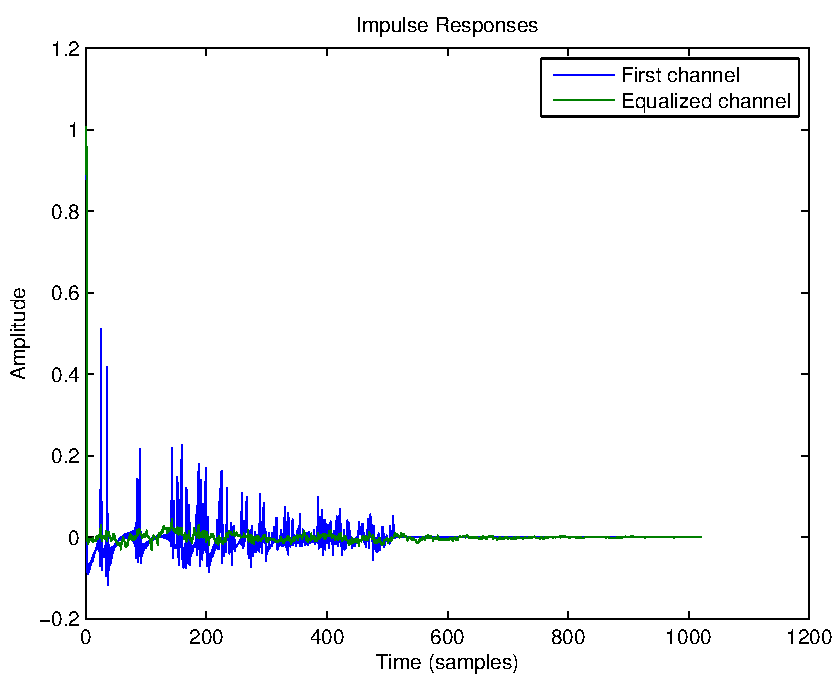
\includegraphics[width=0.475\linewidth]{figs/pdf/ls.pdf}
    \caption{Impulse response of the first channel and the equalized response obtained using the LS algorithm. The NPM of the estimated system is $-30$~dB.}
    \label{fig:ls}
  \end{center}
\end{figure}

	\item[Algorithm] \verb"lsinvfilt()" performs the following operations:

\begin{enumerate}[label=\arabic*.]
    \item Constructs the matrix $\H$ and the vector $\d$.
    \item Computes $\g$ using (\ref{eqn:gls}).
\end{enumerate}
	
	\item[See also] \verb"wls()",  \verb"wls_iterative()", \verb"channel_shortening()"		
\end{enumerate}

% Weighted least squares algorithm
\subsection{Weighted least squares algorithm:~wls()}

\begin{enumerate}[font=\bf, labelindent=\parindent, widest=123456789012, leftmargin=*, align=left]
	\item[Purpose] Design a set of equalization filters given the estimated channel impulse responses.

	\item[Syntax] \verb"[g] = wls(h_hat, Li, k, w)" 

The input and output parameters of \verb"wls()" for an FIR system of size $L \times M$ are summarized below.

\vspace{5pt}
\verb"Input Parameters [size]:" 

\vspace{5pt}
\begin{tabular}[c]{l l l}
  \verb"h_hat" &:& \verb"M impulse responses of length L [L x M]"\\
  \verb"Li" &:& \verb"length of the equalization filters" \\  
  \verb"k" &:& \verb"delay of the target response"\\
  \verb"w" &:& \verb"weighting function [L+Li-1 x 1]"\\
\end{tabular}\\

\vspace{5pt}
\verb"Output Parameters [size]:" 

\vspace{5pt}
\begin{tabular}[c]{l l l}
  \verb"g" &:& \verb"equalization filters [Li x M]" \\
\end{tabular}\\
\vspace{5pt}
	
	\item[Description] 
The weighted LS method \cite{Hofbauer2005} is used for the over-determined cases when the condition C2.1 is violated. The weighted LS solution is found by minimizing
\begin{equation}
J=\|\W(\widehat{\H}\g-\d)\|_2^2, \label{eqn:bew}
\end{equation}
where $\W=\mathrm{diag}\{\w\}$ with $\w=[w(0)~\cdots~w(L+L_i-2)]^T$, and is given by
\begin{equation}
\g=(\W\widehat{\H})^\dag \W\d. \label{eqn:gwls}
\end{equation}
When conditions C2.1 and C2.2 are both satisfied, the solution given by (\ref{eqn:gwls}) is same as that given by (\ref{eqn:gls}) as long as $w(n)\neq 0$, for $n=0,~\cdots~,L+L_i-2$ \cite{Greville1966}.

	\item[Example] The following is an example script (\verb"test_wls.m") that uses \verb"wls()". System identification errors that are generated using the method described in \cite{Zhang2008c} are added to simulated acoustic impulse responses. The NPM of the `estimated' system is -30~dB.

 \lstinputlisting{../test/test_wls.m}

Running the above script (\verb"test_wls.m") will produce Fig.~\ref{fig:wls} that shows the impulse response of the first acoustic channel and the equalized response.
\begin{figure}[htbp]
  \begin{center}
    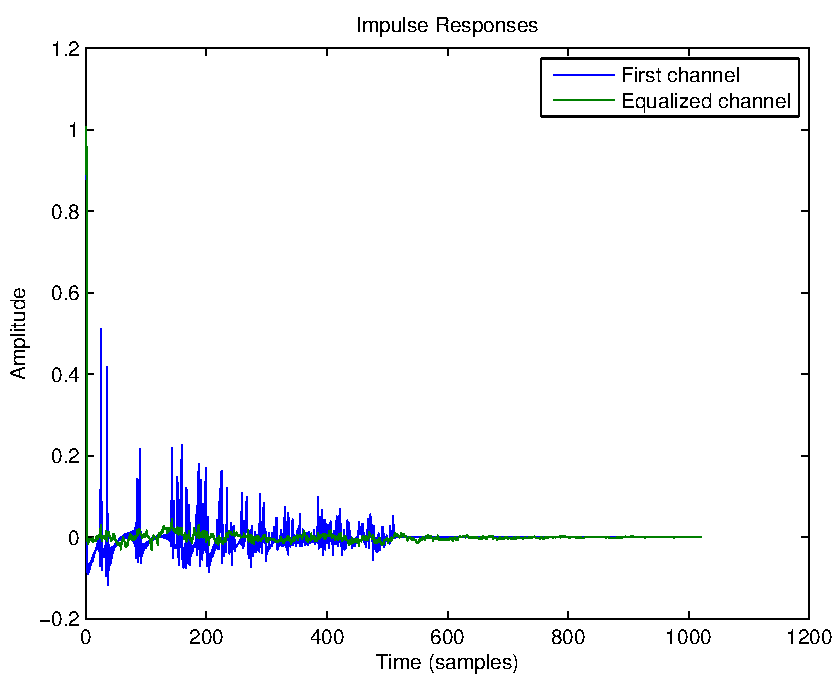
\includegraphics[width=0.475\linewidth]{figs/pdf/wls.pdf}
    \caption{Impulse response of the first channel and the equalized response obtained using the WLS algorithm. The NPM of the estimated system is $-30$~dB.}
    \label{fig:wls}
  \end{center}
\end{figure}

	\item[Algorithm]  \verb"wls()" performs the following operations:

\begin{enumerate}[label=\arabic*.]
    \item Constructs the matrix $\widehat{\H}$ and $\W$, and the vector $\d$.
    \item Computes $\g$ using (\ref{eqn:gwls}).
\end{enumerate}
	
	\item[See also] \verb"ls()",  \verb"wls_iterative()", \verb"channel_shortening()"			
\end{enumerate}

% Iterative weighted least squares algorithm
\subsection{Iterative weighted least squares algorithm:~wls\_iterative()}

\begin{enumerate}[font=\bf, labelindent=\parindent, widest=123456789012, leftmargin=*, align=left]
	\item[Purpose] Design a set of equalization filters given the estimated channel impulse responses.
	
	\item[Syntax] \verb"[g, J] = wls_iterative(h_hat, Li, k, iter, w)" 

The input and output parameters of \verb"wls_iterative()" for an FIR system of size $L \times M$ are summarized below.

\vspace{5pt}
\verb"Input Parameters [size]:" 

\vspace{5pt}
\begin{tabular}[c]{l l l}
  \verb"h_hat" &:& \verb"M impulse responses of length L [L x M]"\\
  \verb"Li" &:& \verb"length of the equalization filters" \\  
  \verb"k" &:& \verb"delay of the target response"\\
  \verb"iter" &:& \verb"number of iterations"\\
  \verb"w" &:& \verb"weighting function [L+Li-1 x 1]"\\
\end{tabular}\\

\vspace{5pt}
\verb"Output Parameters [size]:" 

\vspace{5pt}
\begin{tabular}[c]{l l l}
  \verb"g" &:& \verb"equalization filters [Li x M]" \\
\end{tabular}\\
	
	\item[Description] Equation (\ref{eqn:gwls}) can also be solved iteratively using a conjugate gradient method \cite{Golub1996}.
	
	\item[Example] The following is an example script (\verb"test_wls_iterative.m") that uses \verb"wls_iterative()". System identification errors that are generated using the method described in \cite{Zhang2008c} are added to simulated acoustic impulse responses. The NPM of the `estimated' system is -30~dB.

 \lstinputlisting{../test/test_wls_iterative.m}

Running the above script (\verb"test_wls_iterative.m") will produce the figures shown in Fig.~\ref{fig:wls_iter}. Fig.~\ref{fig:wls_iter_channel} shows the impulse response of the first acoustic channel and the equalized response and Fig.~\ref{fig:wls_iter_J} shows the value of the cost function at each iteration.
\begin{figure}[htbp]
  \begin{center}
    \mbox{
      \subfigure[]{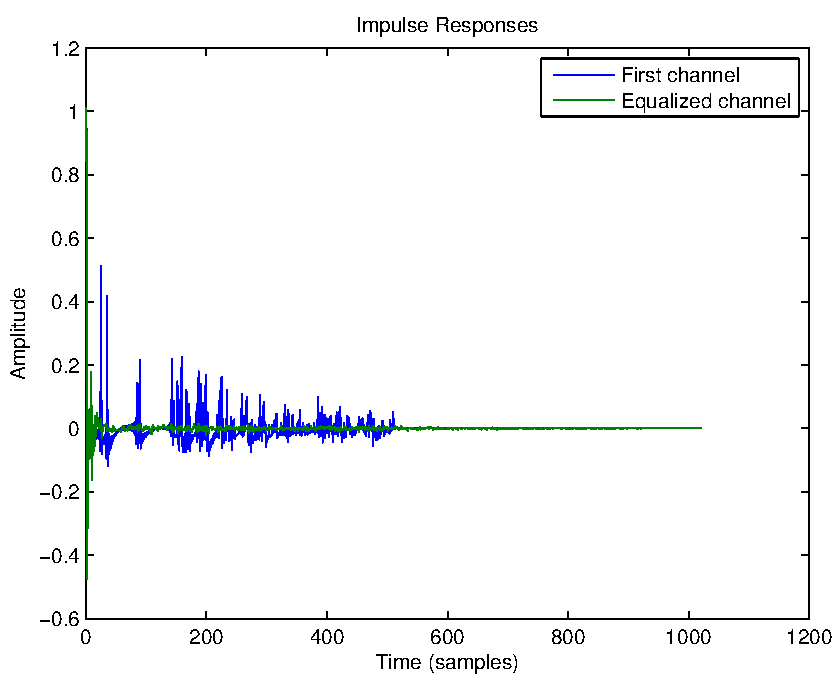
\includegraphics[width=0.475\linewidth]{figs/pdf/wls_iterative.pdf}\label{fig:wls_iter_channel}} \quad
      \subfigure[]{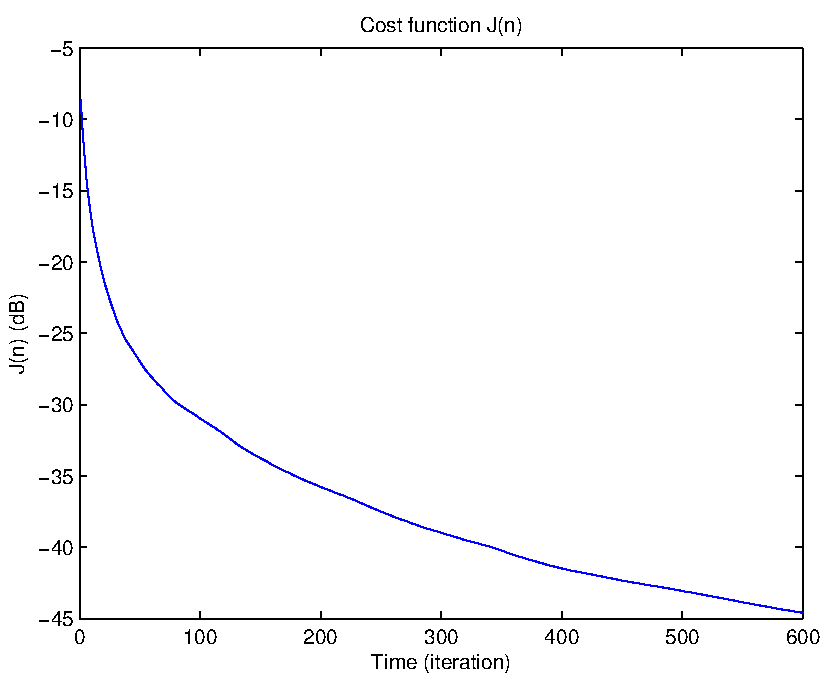
\includegraphics[width=0.475\linewidth]{figs/pdf/wls_iterative_J.pdf} \label{fig:wls_iter_J}}
      }
    \caption{Result obtained using the iterative weighted LS algorithm: (a) impulse response of the first acoustic channel, (b) the value of the cost function at iteration $n$. The NPM of the estimated system is $-30$~dB.}
    \label{fig:wls_iter}
  \end{center}
\end{figure}
	
	\item[Algorithm]  \verb"wls_iterative()" performs the following operations:

\begin{enumerate}[label=\arabic*.]
    \item Initializes $\g$.
    \item Constructs the matrix $\widehat{\H}$ and $\W$, and the vector $\d$.
    \item Performs \verb"iter" iteration to update $\g$.
\end{enumerate}
	
	\item[See also]  \verb"ls()", \verb"wls()", \verb"channel_shortening()"			
\end{enumerate}

% Channel Shortening algorithm
\subsection{Channel shortening algorithm:~channel\_shortening()}

\begin{enumerate}[font=\bf, labelindent=\parindent, widest=123456789012, leftmargin=*, align=left]
	\item[Purpose] Design a set of equalization filters given the estimated channel impulse responses.
	
	\item[Syntax] \verb"[g] = channel_shortening(h_hat, Li, Lw, k)" 

The input and output parameters of \verb"channel_shortening()" for an FIR system of size $L \times M$ are summarized below.

\vspace{-.5em} \begin{verbatim}
Input Parameters [size]:
       h_hat : M impulse responses of length L [L x M] 
       Li    : length of the equalization filters
       k     : delay of the target response
       Lw    : length of the shortened impulse response

Output parameters [size]:
       g     : equalization filters [Li x M] 
\end{verbatim}
	
	\item[Description] Channel shortening techniques \cite{Melsa1996,Martin2005}, which are firstly developed for the equalization of digital communication channels have also been used for acoustic system equalization \cite{Kallinger2006}. The equalization filters can be obtained by  maximizing the generalized Rayleigh quotient:
 \begin{equation}
 \g=\arg\max_{\g}\frac{\g^T\mathbf{A}\g}{\g^T\mathbf{B}\g},
 \label{eqn:cs}
 \end{equation}
where
\begin{align}
\A&=\widehat{\H}^T\mathrm{diag}\{\w_{d}\}^T\mathrm{diag}\{\w_{d}\}\widehat{\H} \label{eqn:mtxB}\\
\B&=\widehat{\H}^T\mathrm{diag}\{\w_{u}\}^T\mathrm{diag}\{\w_{u}\}\widehat{\H} \label{eqn:mtxA}
\end{align}
with
\begin{align}
\w_d &=
[\underbrace{0~\cdots~0}_{\tau}~\underbrace{1~\cdots~1}_{L_w}~0~\cdots~0]^T_{[L+L_i-1 \times 1]}
\nonumber \\
\w_u &= \mathbf{1}_{[L+L_i-1 \times 1]}-\w_d, \nonumber
\end{align}
where $L_w$ defines the length of the non-zero part of the the equalized impulse response.

The solution is the eigenvector corresponding to the largest eigenvalue of the generalized eigenvalue problem \cite{Kallinger2006}
\begin{equation}
\A\g=\lambda\B\g. \label{eqn:cs1}
\end{equation}
	
When conditions C2.1 and C2.2 are both satisfied, (\ref{eqn:cs}) has multiple solutions $\g$ corresponding to $\lambda=\infty$ and the solution given by (\ref{eqn:gls}) is included in the solution space of (\ref{eqn:cs}).

	\item[Example] The following is an example script (\verb"test_channel_shortening.m") that uses \verb"channel_shortening()". System identification errors that are generated using the method described in \cite{Zhang2008c} are added to simulated acoustic impulse responses. The NPM of the `estimated' system is -30~dB.

\lstinputlisting{../test/test_channel_shortening.m}

Running the above script (\verb"test_channel_shortening.m") will produce Fig.~\ref{fig:cs} that shows the impulse response of the first acoustic channel and the equalized response.
\begin{figure}[htbp]
  \begin{center}
    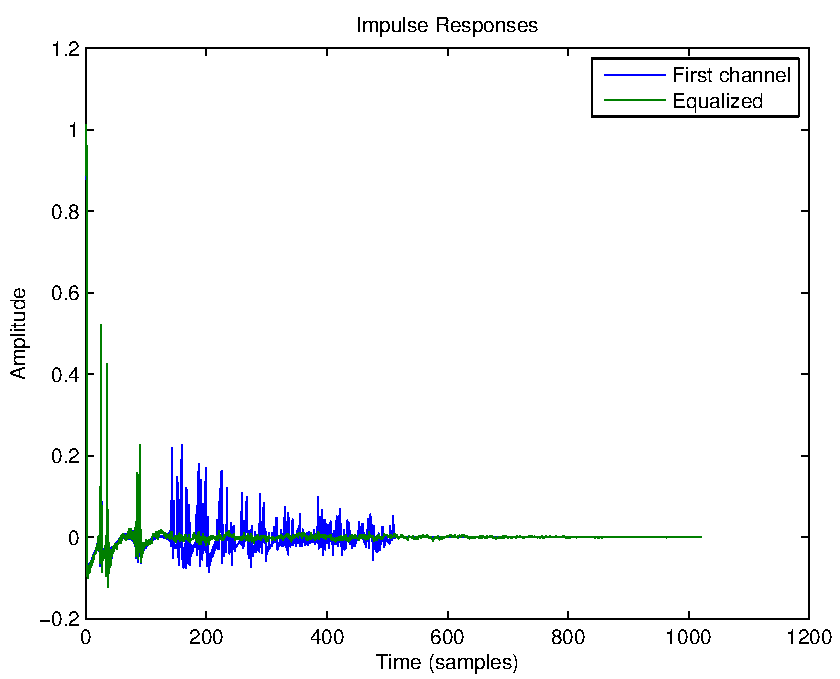
\includegraphics[width=0.475\linewidth]{figs/pdf/cs.pdf}
    \caption{Impulse response of the first channel and the equalized response obtained using the CS algorithm. The NPM of the estimated system is $-30$~dB.}
    \label{fig:cs}
  \end{center}
\end{figure}
	
	\item[Algorithm]  \verb"channel_shortening()" performs the following operations:

\begin{enumerate}[label=\arabic*.]
    \item Constructs the matrix $\A$ and $\B$ defined in (\ref{eqn:mtxA}) and (\ref{eqn:mtxB}), respectively.
    \item Computes the solutions of the generalized eigenvalue problem in (\ref{eqn:cs1}).
    \item Returns the eigenvector that corresponds to the largest eigenvalue $\lambda$.
\end{enumerate}
	
	\item[See also]  \verb"ls()",  \verb"wls()",  \verb"wls_iterative()"
\end{enumerate}

%
% Performance Evaluation and Analyses
%
\section{Performance Evaluation and Analyses}

% Normalized Projection Misalignment
\subsection{Normalized Projection Misalignment:~npm()}

\begin{enumerate}[font=\bf, labelindent=\parindent, widest=123456789012, leftmargin=*, align=left]
	\item[Purpose] Compute the normalized project misalignment (NPM) of the true and the estimate system.
	
	\item[Syntax] \verb"[npm_val] = npm(h, hhat)" 

The input and output parameters of \verb"npm()" are summarized below.

\vspace{-.5em} \begin{verbatim}
Input Parameters [size]:
       h       : true impulse responses [L x M]
       hhat    : estimated impulse responses [L x M]

Output Parameter:
       npm_val : Normalize Projection Misalignment
\end{verbatim}
	
	\item[Description] The performance of BSI is measured by the similarity between true channel impulse responses and estimated ones. Although not available in practice, the true channel impulse response is
available for reference in simulations. The evaluation method should be based on an error measure that is appropriate for the specific problem and independent of how the estimates are derived. Accordingly, define the estimated impulse response for channel $m$ as
\begin{equation}\label{eqn:hhat_ch_LitRev}
    \mathbf{\widehat{h}}_m(n) \, = \, [\widehat{h}_{m,0}(n)~\widehat{h}_{m,1}(n)~\ldots~\widehat{h}_{m,L-1}(n)]^T,
\end{equation}
so that the normalized projection misalignment \cite{Morgan1998} given by
\begin{equation}\label{eqn:NPM}
    \textrm{NPM}(n) \, = \, 20\log_{10}\left( \frac{ \left\|\mathbf{h}-\kappa(n)\widehat{\mathbf{h}}(n)\right\|_2}{\|\mathbf{h}\|_2}\right)~\mathrm{dB}
\end{equation}
can be used as the performance measurement for BSI algorithms, where
\begin{align}
  \mathbf{h} &= [\mathbf{h}_1^T,~\mathbf{h}_2^T,~\ldots,~\mathbf{h}_M^T]^T,\\
  \widehat{\mathbf{h}}(n) &= [\widehat{\mathbf{h}}_1^T(n),~\widehat{\mathbf{h}}_2^T(n),~\ldots,
  ~\widehat{\mathbf{h}}_M^T(n)]^T,  \label{eqn:concat_hhat}
\end{align}
are concatenated vectors of true and estimated channel responses respectively, and
\begin{equation}\label{eqn:kapa}
    \kappa(n) \, = \,
    \dfrac{\mathbf{h}^T\widehat{\mathbf{h}}(n)}{\widehat{\mathbf{h}}^T(n)\widehat{\mathbf{h}}(n)}.
\end{equation}
$\textrm{NPM}(n)$ can be
interpreted as the normalized minimum squared distance from the true channels to the linear manifold of the estimated channels, which is obtained by projecting the former onto the latter \cite{Morgan1998}. Since classic BSI algorithms estimate the channel responses up to an~(unknown) scale factor, the projection error ensures that only the intrinsic misalignment of the channel estimate is taken into account so that the scale factor would not affect the evaluation.

	\item[Algorithm]  \verb"npm()" computes (\ref{eqn:kapa}) and subsequently (\ref{eqn:NPM}).
	
\end{enumerate}

% Magnitude Distortion
\subsection{Magnitude Deviation:~magnitude\_deviation()}

\begin{enumerate}[font=\bf, labelindent=\parindent, widest=123456789012, leftmargin=*, align=left]
	\item[Purpose] Compute the difference between the magnitude response of a true and estimated impulse responses.
	
	\item[Syntax] \verb"[emag emag_freq] = magnitude_deviation(heq, NFFT)" 

The input and output parameters of \verb"magnitude_deviation()" are summarized below.

\vspace{-.5em} \begin{verbatim}
Input Parameters:
       heq       :  equalized impulse response
       NFFT      :  length discrete Fourier transform

Output Parameters:
       emag      :  magnitude deviation
       emag_freq :  magnitude deviation per frequency
\end{verbatim}	
	
	\item[Description] Let us first define the equalized response as
\begin{equation}
	b(i) = \sum_{m=1}^M h_m(i) \ast g_m(i) \quad \mbox{for}\;i=0,\ldots,L+L_i-2.
\end{equation}
We can then define the magnitude deviation as the standard deviation of the equalized magnitude response of $b(i)$, denoted by $B(k)$ ($0 \leq k\leq K-1$), as \cite{Radlovic2000}
\begin{equation} \label{eqn:mag deviation}
	\sigma = \sqrt{\frac{1}{K} \sum_{k=0}^{K-1} \left(10 \log_{10}  \left( \left| B(k) \right|  \right) - \bar{B} \right)^2}
\end{equation}
with
\begin{equation} \label{eqn:mean}
	\bar{B} = \frac{1}{K} \sum_{k=0}^{K-1} 10 \log_{10} \left( \left| B(k) \right| \right).
\end{equation}
This measure is scaling independent and equal to zero for exact equalization.
	
	\item[Algorithm]  \verb"magnitude_deviation()" computes (\ref{eqn:mean}), and subsequently (\ref{eqn:mag deviation}).

	\item[See also] \verb"phase_deviation()"	
\end{enumerate}

% Phase Distortion
\subsection{Phase Distortion:~phase\_deviation()}

\begin{enumerate}[font=\bf, labelindent=\parindent, widest=123456789012, leftmargin=*, align=left]
	\item[Purpose] Compute the difference between the phase response of a true and estimated impulse responses.
	
	\item[Syntax] \verb"[epha epha_freq] = phase_deviation(heq, NFFT)" 

The input and output parameters of \verb"phase_deviation()" are summarized below.

\vspace{-.5em} \begin{verbatim}
Input Parameters:
       heq       :  equalized impulse response
       NFFT      :  length discrete Fourier transform

Output Parameters:
       epha      :  phase deviation
       epha_freq :  phase deviation per frequency
\end{verbatim}		
	
	\item[Description] Linear phase deviation is defined as the deviation of the unwrapped phase from a linear fit to its values and is defined as
\begin{equation} \label{eqn:phase_deviation}
	\Delta = \sqrt{\frac{1}{K} \sum_{k=0}^{K-1} \left(\theta(k) - \bar{\theta} \right)^2}
\end{equation}
where $\bar{\theta}(k)$ is the least squares linear approximation to the phase at frequency bin $k$.

	\item[Algorithm]  \verb"phase_deviation()" computes (\ref{eqn:phase_deviation}).
	
	\item[See also]  \verb"magnitude_distortion()"			
\end{enumerate}
	
% GMC_ST
\subsection{Generalized Multichannel Clustering:~gmc\_st()}

\begin{enumerate}[font=\bf, labelindent=\parindent, widest=123456789012, leftmargin=*, align=left]
	\item[Purpose] The generalized multichannel clustering algorithm, proposed in \cite{Khong2008} efficiently extracts clusters of near-common zeros within a specified pairwise distance in the $z$-plane. Using this algorithm it is possible to quantify the number of common zeros that exist in acoustic systems.
	
	\item[Syntax] \verb"[ClustMtx] = gmc_st(zr, tol)"

The input and output parameters of \verb"gmc_st()" are summarized below.

\vspace{-.5em} \begin{verbatim}
Input Parameters [size]:
       zr       : zeros of the channel impulse 
                  responses [L-1 x M]
       tol      : tolerence

Output Parameters:
       ClustMtx : a matrix containing number of 
                  clusters-by-cluster members
\end{verbatim}
	
	\item[Description]
	
For a multichannel system, clusters of near-common zeros must satisfy two conditions:
\begin{enumerate}[label=\roman*.]
	\item The number of zeros within each cluster must correspond to the number of channels for that system  with each channel contributing exactly one zero.
	\item All possible pairs of zeros in a cluster must lie within a vicinity $\delta$ in terms of their Euclidean distances where $\delta\geq0$ is defined as the tolerance. 
\end{enumerate}
Condition (i) results from the definition of zeros being near common across all channels. Condition~(ii) defines the closeness between pairs of near-common zeros. It is worthwhile noting that the channel disparity depends on these pairwise distances~\cite{Fijalkow1996} and any zero can be a member of more than one cluster. As explained in \cite{Khong2008}, this implies that classical clustering algorithms such as the $k$- and $c$-means algorithms~\cite{Jain99} cannot be employed. An illustrative example of two clusters of near-common zeros in the $z$-plane for a three-channel system satisfying the above conditions is shown in Fig.~\ref{Fig:clusteringExamples}. Symbols $\triangle$, $\Box$ and $\circ$ represent zeros for each channel and they lie within pairwise $\delta$ vicinity from each other.
	
Extraction of clusters of near-common zeros in a multichannel system involves the computation of the Euclidean distances between any pair of zeros from different channels. A novel approach to compute these distances between any two channels was proposed in \cite{Khong2008}. It is assumed that each of these high order polynomials has been factorized using efficient factorization algorithms presented in~\cite{Sitton2003}. Defining $\mathbf{h}_m=[h_{m,0}~~h_{m,1}~~\ldots~~h_{m,L-1}]^T$ as the $m$th channel impulse response of length $L$ we can then express for $z=e^{i2\pi f}$ and $i=\sqrt{-1}$,
\begin{eqnarray}
H_m(z) = h_{m,0}+\ldots+h_{m,L}z^{-L+1} =
K\prod^{L-1}_{p=1}\big(z-z_m(p)\big), \nonumber
\end{eqnarray}
where $f$ is the normalized frequency and $K$ is the gain constant. The term $z_{m}(p)=x_{m}(p)+iy_{m}(p)$ is the $p$th zero and its location in the $z$-plane is defined by $x_m(p)$ and $y_m(p)$ along the real and imaginary axis of the unit circle respectively. It has been shown~\cite{Hughes2004} that as $L$ increases, the radii of these zeros tend toward unity while their angles tend toward a uniform distribution.

The rate of convergence for adaptive BSI algorithms reduces with the reduction of Euclidean distances between the zeros~\cite{Lin2006}. In addition, the relationship between channel disparity and pairwise distances of the zeros has been established in~\cite{Fijalkow1996}. To quantify these pairwise distances, we introduce an $L-1 \times L-1$ dissimilarity matrix $\mathbf{D}_{\{m,n\}}$ defined between channels $m$ and $n$ where the $p$th row and $q$th column element is given by
\begin{eqnarray} D_{\{m,n\}}(p,q) \hspace{-8pt} &=& \hspace{-8pt}
|z_{m}(p)-z_{n}(q)| \nonumber \\
~ \hspace{-8pt} &=& \hspace{-8pt}
\sqrt{\big[x_{m}(p)-x_{n}(q)\big]^2+\big[y_{m}(p)-y_{n}(q)\big]^2}~
\nonumber \\
~ &~& ~ \label{Eqn:distMtx}
\end{eqnarray}
for $p,q=1,\ldots,L$ and $m\neq n$. Unless the zeros are exactly common,~(i)~the diagonal elements of $\mathbf{D}_{\{m,n\}}$ are non-zero and (ii)~$\mathbf{D}_{\{m,n\}}$ is not symmetric. We next define two $L\times1$ vectors
\begin{eqnarray}
\mathbf{z}_m &=& [z_{m}(1)~z_{m}(2)~\ldots~z_{m}(L-1)]^T,
\label{Eqn:z_m}\\
\mathbf{z}_n &=& \big[z_n(1)~z_n(2)~\ldots~z_n(L-1)\big]^T
\label{Eqn:z_n}
\end{eqnarray}
containing $L$ zeros of the $m$th and $n$th channel respectively. Defining
$\mathbf{\widetilde{Z}}_m=\mathbf{Z}_m\odot\mathbf{Z}_m$ with
$\odot$ being the Hadamard product, $\mathbf{Z}_m =
\mathbf{z}_m\mathbf{1}^T$, $\mathbf{Z}_n = \mathbf{1}\mathbf{z}^T_n$
and $\mathbf{1}_{[L-1 \times 1]}=[1~~1~~\ldots~~1]^T$, computation of~(\ref{Eqn:distMtx}) for all $p$ and $q$ can be efficient using
\begin{equation}
\mathbf{D}_{\{m,n\}}=
\Big[\Big|\mathbf{\widetilde{Z}}_m-2\mathbf{z}_m\mathbf{z}^T_n+\mathbf{\widetilde{Z}}_n\Big|\Big]^{\circ\frac{1}{2}},
\label{Eqn:distMtxComp}
\end{equation}
with $[\cdot]^{\circ\frac{1}{2}}$ and $|\cdot|$ being the Hadamard square root and elemental absolute respectively. To illustrate the validity of~(\ref{Eqn:distMtxComp}), we write \footnotesize
\begin{eqnarray}
\mathbf{\widetilde{Z}}_m-2\mathbf{z}_m\mathbf{z}^T_n+\mathbf{\widetilde{Z}}_n
\hspace{-2.5cm} &~&~ \nonumber
\\
\hspace{-2.5cm} &=& \left[
\begin{array}{ccc}
\big(z_m(1)-z_n(1)\big)^2 & \cdots       & \big(z_m(1)-z_n(L-1)\big)^2 \\
\vdots                    & \ddots       & \vdots \\
\big(z_m(L-1)-z_n(1)\big)^2 & \cdots       & \big(z_m(L-1)-z_n(L-1)\big)^2 \\
\end{array}
\right].
\end{eqnarray}
\normalsize Let $a=x_m(p)-x_n(q)$ and $b=y_m(p)-y_n(q)$. Invoking Euler's identity $a+ib=re^{i\theta}$ where $r=\sqrt{a^2+b^2}$ and $\theta=\mathrm{tan}^{-1}(b/a)$, we have $\big|(a+ib)^2\big|=\big|r^2e^{i2\theta}\big| = r^2$, from which we obtain the important result \footnotesize
\begin{eqnarray}
\mathbf{D}_{\{m,n\}} \hspace{-0.3cm} &=& \hspace{-0.3cm}
\Big[\big|\mathbf{\widetilde{Z}}_m-2\mathbf{z}_m\mathbf{z}^T_n+\mathbf{\widetilde{Z}}_n\big|\Big]^{\circ\frac{1}{2}}
\nonumber
\\
~ \hspace{-0.3cm} &=& \hspace{-0.3cm} \left[
\begin{array}{ccc}
\sqrt{|(z_m(1)-z_n(1))^2|} & \cdots           &\sqrt{|(z_m(1)-z_n(L-1))^2|} \\
\vdots                     & \ddots           &\vdots   \\
\sqrt{|(z_m(L-1)-z_n(1))^2|} & \cdots           & \sqrt{|(z_m(L-1)-z_n(L-1))^2|} \\
\end{array}
\right] \nonumber
\end{eqnarray}
\normalsize hence verifying the validity of~(\ref{Eqn:distMtxComp}). For $m\neq n$, since all pairwise distances are computed only once, no computational redundancy occurs making this computation efficient.
	
\begin{figure}[t]
\centering
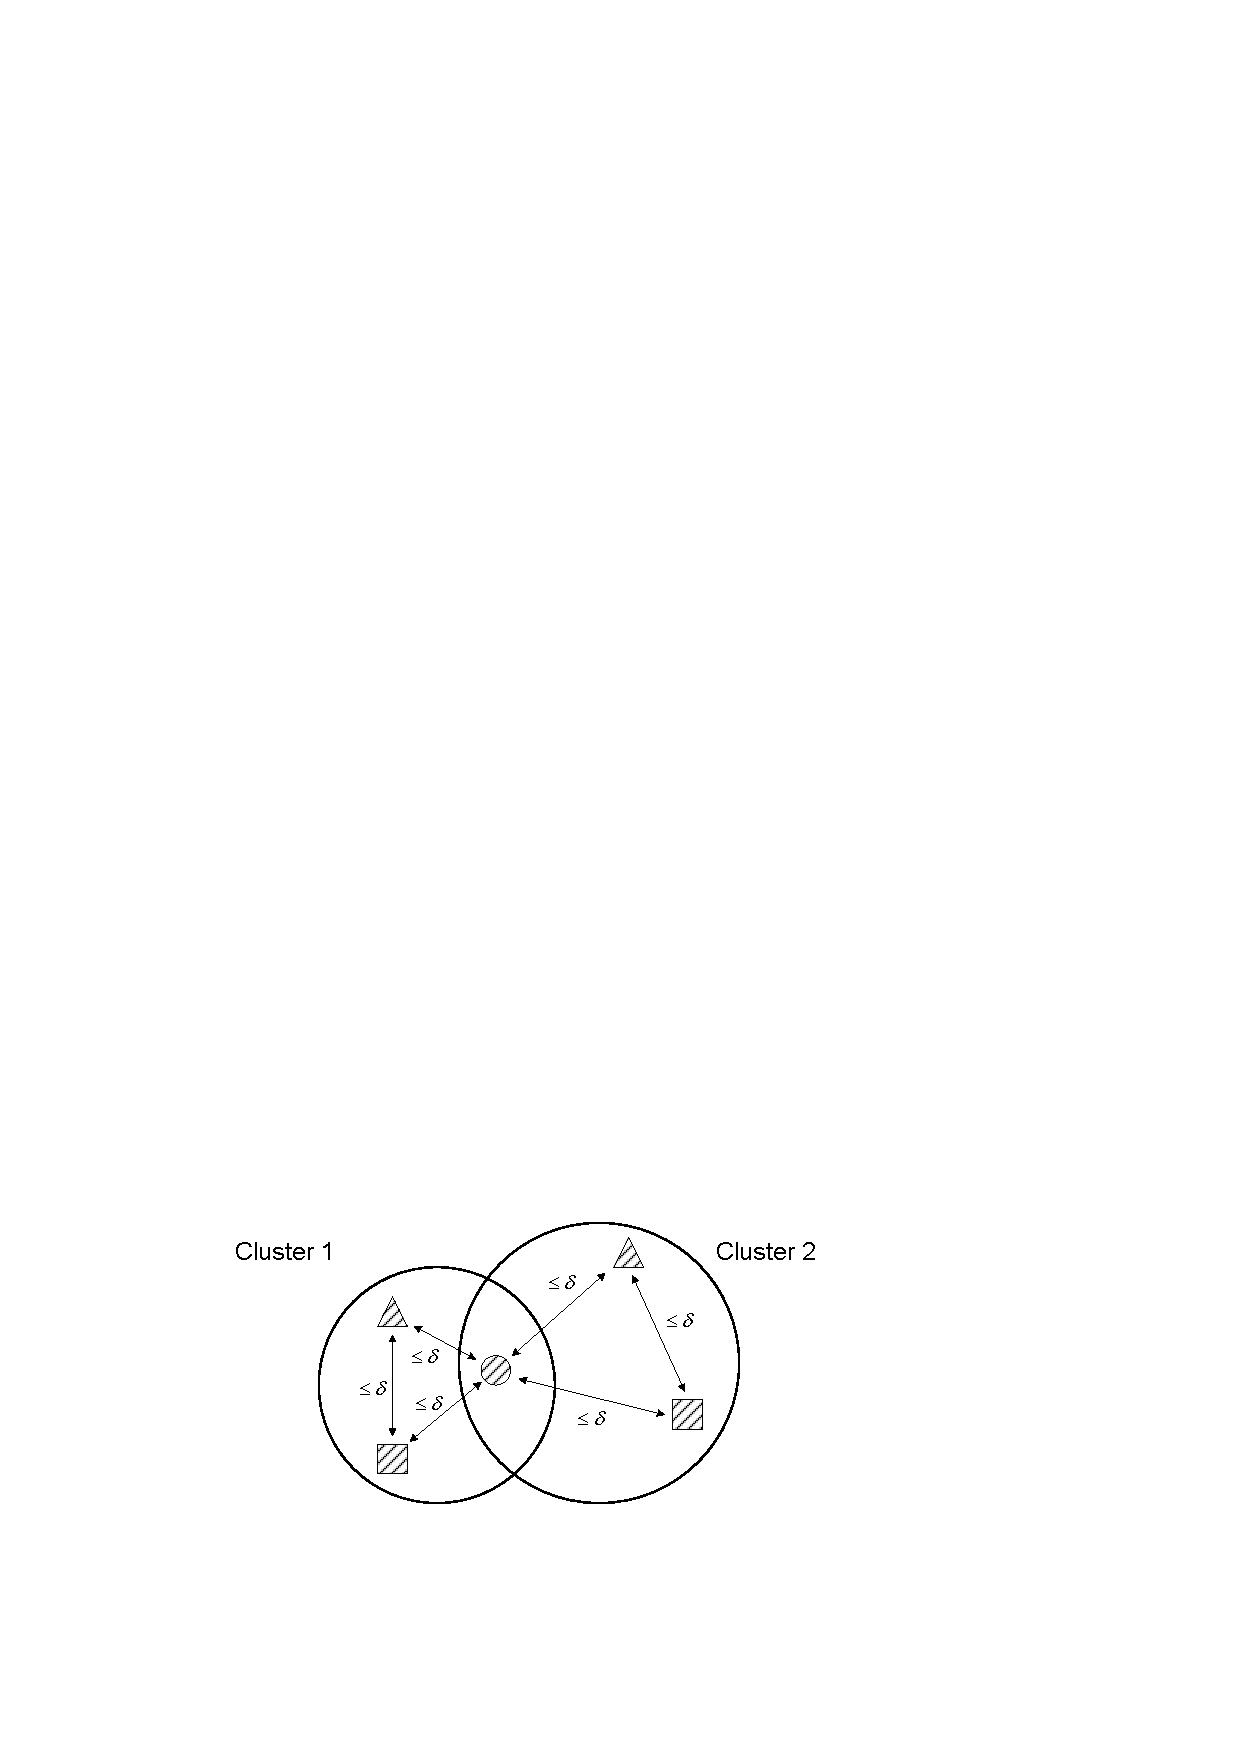
\includegraphics[scale=0.65]{figs/pdf/clusteringExamples.pdf}
\caption{\footnotesize An example of two clusters for a three-channel system in the $z$-plane.}
\label{Fig:clusteringExamples}
\end{figure}
	
Employing $\mathbf{D}_{\{m,n\}}$ between any two out of $M$ channels, consider the case where there are $c_{mn}$ clusters of near-common zeros between channels $m$ and $n$. We next define a sub-cluster group matrix $\boldsymbol{\mathcal{C}}_{\{m,n\}}$ containing these $c_{mn}$ clusters. This $c_{mn}\times 2$ matrix can be obtained by searching within elements in $\mathbf{D}_{\{m,n\}}$ for indices $p$ and $q$ such that
\begin{equation}
\boldsymbol{\mathcal{C}}_{\{m,n\}}= \displaystyle\arg
D_{\{m,n\}}(p,q)\leq\delta \label{Eqn:clusterspwch}
\end{equation}
is satisfied. We next denote $c_t$ as the total number of clusters for the $M$-channel system. We define cluster matrix $\boldsymbol{\mathcal{C}}_{\{1:M\}}$ of dimension $c_t\times M$ for the whole system where each row contains a cluster with $M$ elements each containing indices corresponding to elements in $\{\mathbf{z}_1~~\mathbf{z}_2~~\ldots~~\mathbf{z}_M\}$ for the respective channels $1$ to $M$. We employ~(\ref{Eqn:clusterspwch}) across each pair of channels selected from $M$. The aim of the generalized multichannel clustering~(GMC) algorithm is to obtain $\boldsymbol{\mathcal{C}}_{\{1:M\}}$ using sub-cluster groups $\boldsymbol{\mathcal{C}}_{\{m,n\}}$.

	\item[Example] The following is an example script (\verb"test_gmc.m") of running \verb"gmc_st()".

\lstinputlisting{../test/test_gmc.m}
 		
	\item[Algorithm] The GMC Search-and-Trim (GMC-ST) algorithm first computes $\mathbf{D}_{\{m,n\}}$
for all possible pairs of channels with $m=1, \ldots,M-1$ and $n=m+1$. This employs~(\ref{Eqn:distMtxComp}) a total of $0.5M(M-1)$ times. Invoking~(\ref{Eqn:clusterspwch}), this algorithm then aims to extract $\boldsymbol{\mathcal{C}}_{\{1:M\}}$ from these $0.5M(M-1)$ sub-cluster groups $\boldsymbol{\mathcal{C}}_{\{m,n\}}$ using an efficient search technique. This is achieved by first selecting the sub-cluster group
\begin{equation}
\boldsymbol{\mathcal{C}}_{\{m_s,n_s\}}=
\min_{c_{mn}}\Big\{\boldsymbol{\mathcal{C}}_{\{1,2\}}~~
\boldsymbol{\mathcal{C}}_{\{1,3\}}~...~\boldsymbol{\mathcal{C}}_{\{M-1,M\}}\Big\},
\label{Eqn:C_ms_ns}
\end{equation}
having the smallest $c_{mn}$ as a reference group. This is equivalent to finding the two channels $m_s$ and $n_s$ having the smallest number of sub-clusters. Since near-common zeros must satisfy condition~(i), GMC-ST begins its search from $\boldsymbol{\mathcal{C}}_{\{m_s,n_s\}}$. For each row of $\boldsymbol{\mathcal{C}}_{\{m_s,n_s\}}$, GMC-ST initializes a row vector $\mathbf{R}=[r(1)~\ldots~r(M)]$ with only two non-empty elements $r(m_s)=p$ and $r(n_s)=q$ where $p$ and $q$ are two elements obtained from each row in $\boldsymbol{\mathcal{C}}_{\{m_s,n_s\}}$. The next stage is to search, for row vector $\mathbf{r}$ of $\mathbf{R}$, the remaining $M-2$ empty elements. This search space is confined within 
$\big\{\boldsymbol{\mathcal{C}}_{\{1,2\}}~~\boldsymbol{\mathcal{C}}_{\{1,3\}}~...~\boldsymbol{\mathcal{C}}_{\{M-1,M\}}\big\}$ excluding $\boldsymbol{\mathcal{C}}_{\{m_s,n_s\}}$ since, from~(\ref{Eqn:clusterspwch}), only zeros within these groups are all within tolerance $\delta$. If $k$ elements are found, then $\mathbf{R}$ is updated as
\begin{equation}
\mathbf{\widetilde{R}}= \mathbf{1}_{[k\times1]}\mathbf{r}, \qquad
\mathbf{R}=[\mathbf{\widetilde{R}}^T~~\mathbf{R}^T]^T,
\label{Eqn:updateR}
\end{equation}
where $\mathbf{1}_{[k\times1]}=[1~\ldots~1]^T$. This implies that the zeros belong to $k$ different clusters. The trimming process then ensures that all pairwise elements for each row in $\mathbf{R}$ can be found within the search space 
$\big\{\boldsymbol{\mathcal{C}}_{\{1,2\}}~~\boldsymbol{\mathcal{C}}_{\{1,3\}}~...~\boldsymbol{\mathcal{C}}_{\{M-1,M\}}\big\}$ in order to satisfy condition~(ii). If this condition is violated, the entire row is deleted and the search-and-trim process is repeated until every element in each row of $\mathbf{R}$ is found or all rows have been deleted.

\end{enumerate}

% EDC
\subsection{Energy Decay Curve and Derived Measures:~edc()}

\begin{enumerate}[font=\bf, labelindent=\parindent, widest=123456789012, leftmargin=*, align=left]
	\item[Purpose] The energy decay curve (EDC) is a measure of the decay of an RIR or EIR, shown in~\cite{Schroeder1965} to be identical to the ensemble average decay of a system excited with white noise. It is inversely proportional to reverberation time~\cite{Kuttruff2000} and is used in the derivation of a set of objective measures for an RIR.
	
	\item[Syntax] \verb"[decay,...] = edc(h,fs,...)"

The input and output parameters of \verb"edc()" are summarized below. If no outputs are specified then the EDC is plotted.

\vspace{-.5em} \begin{verbatim}
Input Parameters [size]:
       h    : room impulse response 
              [L-1 x 1]
       fs   : Sampling frequency (Hz)
       meas : [Optional] Any number of strings containing
              `Txx': Reverberation time (ms)
              `Cxx': Clarity index (early-to-late ratio) (dB)
              `Dxx': Deutlichkeit (early-to-total sound energy) (dB)
              where xx specifies the argument in dB for `Txx' and in 
              ms for `Cxx' and `Dxx'. Meas can also contain cell arrays.

Output Parameters [size]:
       decay: Normalized energy decay curve in dB
              [Lx1]        	
       meas : Measures in order of input argument
\end{verbatim}
	
	\item[Description]
	The EDC of an RIR is calculated by~\cite{Schroeder1965}
\begin{equation}
	\textrm{EDC}(i)=\frac{1}{\|\mathbf{h}\|^2_2}\sum_{n=i}^{L-1}h^2(n),~i\in \{0,1,\dots,L-1\}.
\end{equation}
The measure  $\mathrm{T}_{60}$ the time for the energy decay curve (EDC) of an RIR to drop by $60~\textrm{dB}$ of its maximum value~\cite{Kuttruff2000}. Similarly, the measure $\mathrm{T}_{30}$ is commonly used in the context of EIRs.

The early-to-late reverberation reverberation ratio (ELR), also known as the Clarity Index, is highly-correlated with the intelligibility of reverberant speech and is defined as~\cite{Kuttruff2000}
\begin{align}
	\mathrm{C}_{n_e}&=\frac{\sum_{n=0}^{n_e}h^2(n)}{\sum_{n=n_e+1}^{\infty}h^2(n)}\\
	  		 	    &=\frac{\textrm{EDC}(0)-\textrm{EDC}(n_e+1)}{\textrm{EDC}(n_e+1)}.
\end{align}

Deutlichkeit, the early-to-total sound energy, is defined as~\cite{Kuttruff2000}
\begin{align}
	\mathrm{D}_{n_e}&=\frac{\sum_{n=0}^{n_e}h^2(n)}{\sum_{n=0}^{\infty}h^2(n)}\\
	  		 	    &=\frac{\textrm{EDC}(0)-\textrm{EDC}(n_e+1)}{\textrm{EDC}(0)},
\end{align}

The constant $n_e$ is often chosen to be $n_e=50~\textrm{ms}\cdot f_\mathrm{s}$. EDC, $\mathrm{C}_{n_e}$ and $\mathrm{D}_{n_e}$ outputs are expressed on a log scale.
\end{enumerate}

%%%%%%%%%
\section{Auxiliary Functions}

\subsection{Generate Data: generate\_data()}
\begin{enumerate}[font=\bf, labelindent=\parindent, widest=123456789012, leftmargin=*, align=left]
	\item[Purpose] This function computes the room impulse responses and generates WGN data with additive noise.
		
	\item[Syntax] \verb"[h, x, tau] = generate_data(M, L, fs, air, N, SNR)" 

The input and output parameters of \verb"generate_data()" are summarized below.

\vspace{-.5em} \begin{verbatim}
Input Parameters:
       M      : number of channels
       L      : filter length
       fs     : sample frequency
       air    : struct with acoustic impulse response 
                parameters
       N      : data length
       SNR    : average signal to noise ratio across
                sensor signals (optional: default 30 dB)

Output Parameters:
       h      : acoustic impulse responses
       x      : noisy and reverberant sensor signals
\end{verbatim}		
	
	%\item[Description] ...
		
\end{enumerate}

\subsection{Generate System Identification Errors: generate\_sie()}
\begin{enumerate}[font=\bf, labelindent=\parindent, widest=123456789012, leftmargin=*, align=left]
	\item[Purpose] This function generates system identification errors.
		
	\item[Syntax] \verb"[ie]  = generate_sie(h, npm, mode, T60, fs)" 

The input and output parameters of \verb"generate_sie()" are summarized below.

\vspace{-.5em} \begin{verbatim}
Input Parameters:
       h      : system impulse responses
       npm    : desired NPM level in dB
       mode   : the shape of errors. Three options are 
                'wgn'  white Gaussian noise like errors;
                'prop' WGN but proportional to h;
                'damp' damping errors, damping factor same as h
       T60    : the reverberation time of h, only needed for
                generating damping errors
       fs     : sampling frequency, only needed for generating 
                damping errors (optional: default 8000)

Output Parameters:
       ie     : the representation of identification errors
\end{verbatim}		
	
	%\item[Description] ...
		
\end{enumerate}

\subsection{Remove Direct-Path Propagation: rdp()}
\begin{enumerate}[font=\bf, labelindent=\parindent, widest=123456789012, leftmargin=*, align=left]
	\item[Purpose] This function removes the smallest direct-path propagation of room impulse responses generated by image method.
		
	\item[Syntax] \verb"[h, dl]  = rdp(h_unc, tau, stat)" 

The input and output parameters of \verb"rdp()" are summarized below.

\vspace{-.5em} \begin{verbatim}
Input Parameters:
       h_unc   : original room impulse responses
       tau     : TDOAs with respect to first sensor in
                 (fractional) samples
       seed    : seed for generating padding random taps

Output Parameters:
       h       : updated room impulse responses
\end{verbatim}		
	
	%\item[Description] ...
		
\end{enumerate}

\subsection{Sensor Positions of a Uniform Linear Array: ula\_pos()}
\begin{enumerate}[font=\bf, labelindent=\parindent, widest=123456789012, leftmargin=*, align=left]
	\item[Purpose] This function positions a ULA such that its centroid is in the middle of the room. 

	\item[Syntax] \verb"micPos = ula_pos(micSpc,micNum,CenPos)" 

The input and output parameters of \verb"ula_pos()" are summarized below.

\vspace{-.5em} \begin{verbatim}
Input Parameters:
       micSpc  : microphone spacing
       micNum  : number of microphones
       CenPos  : center position of the array

Output Parameters:
       micPos  : a 3-by-micNum vector containing mic positions 
\end{verbatim}		
	
	%\item[Description] ...
		
\end{enumerate}

%
% Conclusions
%
\section{Conclusions}
This BSIE toolbox contains various state-of-the-art algorithms for blind system identification and system equalization. In addition, it contains performance evaluation and analyses functions.

%
% Acknowledgment 
%
\section*{Acknowledgment}
The authors would like to thank Mr. Mark Thomas for proofreading the manuscript.

%
% References
%
\bibliographystyle{IEEEtran}
%\bibliography{IEEEabrv,references}
\bibliography{IEEEabrv,/Users/mark/Work/Project/Bibliography/SAPBibTex/sapref}
%\bibliography{IEEEabrv,/Users/ehabets/CVS/SAP/SAPBibTex/sapref}

\end{document}